\documentclass[a4paper, draft]{report}
\pagestyle{headings}
\author{C. Bohr}

\title{Feed-forward neuronal networks - an introduction}

\usepackage{amsmath,amsthm, amsfonts,amscd, amssymb, a4}
\usepackage[final]{graphicx}
\usepackage[final]{listings}
\usepackage{bbm}
\usepackage{empheq}
\usepackage{caption}
\usepackage{hyperref}

\renewcommand\lstlistingname{Algorithm}
\captionsetup[lstlisting]{singlelinecheck=false, margin=0pt, font={sf},labelsep=space,labelfont=bf}



% Numbering

\numberwithin{section}{chapter}
\numberwithin{equation}{chapter}

% Theorem environments

%% \theoremstyle{plain} %% This is the default
\newtheoremstyle{own}
    {3pt}                    % Space above
    {3pt}                    % Space below
    {\itshape}                   % Body font
    {}                           % Indent amount
    {\scshape}                   % Theorem head font
    {.}                          % Punctuation after theorem head
    {.5em}                       % Space after theorem head
    {}  % Theorem head spec (can be left empty, meaning ‘normal’)
    
\theoremstyle{own}
\newtheorem{thm}{Theorem}[section]
\newtheorem{cor}[thm]{Corollary}
\newtheorem{lem}[thm]{Lemma}
\newtheorem{prop}[thm]{Proposition}
\newtheorem{ax}{Axiom}[section]

%% \theoremstyle{definition}
\newtheorem{defn}{Definition}[section]

%% \theoremstyle{remark}
\newtheorem{rem}{Remark}[section]
\newtheorem*{notation}{Notation}
\newtheorem{algorithm}{Algorithm}[section]
\theoremstyle{remark}
\newtheorem{example}{Example}[section]

% Fix alignments

% \setlength{\parindent}{0cm}

\newcommand*\widefbox[1]{\fbox{\hspace{4em}#1\hspace{4em}}}
\newcommand*\fullbox[1]{\framebox[\columnwidth]{#1}}

%  Math definitions

% Fields
\newcommand{\R}{\mathbb{R}}
\newcommand{\C}{\mathbb{C}}
\newcommand{\Z}{\mathbb{Z}}
\newcommand{\Q}{\mathbb{Q}}
\newcommand{\N}{\mathbb{N}}
\newcommand{\quat}{\mathbb{H}}

%Groups 
\newcommand{\Lo}{\mathbf{O}(3,1)}
\newcommand{\SL}{\mathbf{SL}}
\newcommand{\SU}{\mathbf{SU}}
\newcommand{\Spin}{\mathbf{Spin}}
\newcommand{\Pin}{\mathbf{Pin}}
\newcommand{\SO}{\mathbf{SO}}
\newcommand{\Poincare}{\mathcal{P}}
\newcommand{\Poincarecov}{\widetilde{\mathcal{P}}}
\newcommand{\Poincareprop}{\widetilde{\mathcal{P}}_+^{\uparrow}}
\newcommand{\Aut}{\mathrm{Aut}}

% Rings
\newcommand{\End}{\mathrm{End}}
\newcommand{\CCl}{\mathbb{C}\mathrm{l}}
\newcommand{\Cl}{\mathrm{Cl}}
\newcommand{\Mat}{\mathrm{Mat}}

% Lie algebras

\newcommand{\spin}{\mathfrak{spin}}
\newcommand{\so}{\mathfrak{so}}
\newcommand{\su}{\mathfrak{su}}
\newcommand{\slc}{\mathfrak{sl}}

%Three-vectors
\newcommand{\xt}{\mathbf{x}}
\newcommand{\yt}{\mathbf{y}}
\newcommand{\pt}{\mathbf{p}}
\newcommand{\nt}{\mathbf{n}}
\newcommand{\sigmat}{\mathbf{\sigma}}

% Vector spaces
\newcommand{\Hil}{\mathcal{H}}

% Other
\newcommand{\calE}{\mathcal{E}}
\newcommand{\calD}{\mathcal{D}}
\newcommand{\calF}{\mathcal{F}}
\newcommand{\calP}{\mathcal{P}}
\newcommand{\Fock}{\mathcal{F}}
\newcommand{\Op}{\mathrm{Op}}

\DeclareMathOperator{\per}{per}
\DeclareMathOperator{\sign}{sgn}
\DeclareMathOperator{\logit}{logit}

\begin{document}
\maketitle

\tableofcontents



%%%%%%%%%%%%%%%%%%%%%%%%%%%%%%%%%%%%%%%%%%%%%%
%% Probability
%%%%%%%%%%%%%%%%%%%%%%%%%%%%%%%%%%%%%%%%%%%%%%
\chapter{Statistics and neuronal networks}

Learning neuronal networks is hard. Of course getting a first exposure to neuronal networks and getting a first example for image recognition set up and running has become very easy thanks to the
plethora of good (and not so good) tutorials available in the net and thanks to frameworks like Theano or Tensorflow. However, if that is not enough and you start digging deeper and trying to understand
why and how neuronal networks actually work, it turns out that things quickly get much more complicated than that. You will very soon be confronted with - at times non-trivial - mathematics from branches like statistics, information theory, linear algebra and real analysis.

The purpose of these notes is guide you on that journey and to provide a bit more detail behind the usual introductory level crash courses. We will mainly focus on the area of {\em feed forward networks} used for {\em supervised learning}. Some other classes of networks like energy based models and some methods from unsupervised learning are presented in more detail on my blog \url{www.leftasexercise.com}.


Most of the mathematics that we will need is somehow related to the field of mathematical statistics - let us first try to understand where this relation comes from.

Many neuronal networks are designed to excel at {\em classification tasks}. As an example, suppose you wanted to design and train a neuronal network that, given data about an animal, classifies the animal as either a bird or some other animal (called a ``non-bird'' for convenience). So our starting point
is a set modelling all possible objects that could be presented to the network. How exactly we model this set is not so important, more important is that in general, the network will not have access to all the data about the animal, but only to certain attributes of elements in the set called {\em features}. So
there could be an attribute which we call $X$ that is defined as
$$
X_1 = \text{the animal can fly}
$$
taking values in $\{0,1\}$. Another data point the network could get is
$$
X_2 = \text{length of animal in cm}
$$
taking values in $\R^+$ and so forth. More generally, we assume that on the set of all possible objects, we have certain functions $X_i$ taking values in, say, the real numbers. Based on these numbers, the network will then try to take a decision whether a given animal is a bird or not. Thus we do not have to deal directly with our space of objects, but use the functions $X_i$ as primary objects.

If the network had a chance to look at every possible animal, this would be easy, even though it would cost a lot memory - we could simply remember all possible combinations of features and for each feature, store the correct answer. In reality however, this does not work. Instead, we have access to a small subset of data - a {\em sample} for which we can evaluate the $X_i$. Based on this subset, we then have to derive a model which gives the right answer in as many cases as possible. Thus we try to make a statement about the full space of things that could be 
presented to our network for classification based on a small sample. 

This is where probabilities come into play very naturally. We need to assume that our sample has been chosen randomly, but still we need to make assertions about the full set. This is exactly what {\em inferential statistics} is doing. The fact that our sample is chosen randomly turns our $X_i$ into {\em random variables}. Similarly, the variable
$$
Y = \text{is a bird}
$$
taking values in $\{0,1\}$ is a random variable, and we try to gain information on the distribution of $Y$ across the full population based on its values on a given set of labelled samples, i.e. a set of samples where $Y$ is known. Thus $Y$ would represent the {\em labels} or {\em targets} in the language of neuronal networks. Applying the methods of statistical inference to this situation would typically start by chosing a statistical model and than using estimators or hypothesis testing to make deductions.

Apart from the fact that we have to derive information on the full population based on a sample, there is another reason why probabilities appear naturally in the theory of machine learning. In many cases, the available input - being a reduction of the full set of data - is not sufficient to classify the sample with full certainty. To see this, let us go back to our examples. How would you derive the property ``bird'' from the given data ``can fly'' and ``length''? Not all animals than can fly are birds - and not all birds can fly. So we have to try to distinguish for instance a butterfly from a hummingbird based on the length.  The smallest hummingbird - a bee hummingbird - is about 5 cm in length. The largest known butterfly - the Queen's Alexandra birdwing - can be as long as 8 cm (both informations taken from Wikipedia). Thus our data is not sufficient to clearly distinguish butterflies and birds in all cases. However, very small birds and very large butterflies have one thing in common - they are rare. So chances are that a given animal that can fly and is larger than 5 cm is actually a bird (yes, there are bats....). In other words, if again $Y$ denotes the variable which is 1 on birds and 0 on all other animals, we can in general not hope that $Y$ is a function of the $X_i$, but we can hope that given some values of the $X_i$, the probability $P(Y=1)$ to be a bird depends on the $X_i$. In other words, using the language of {\em conditional probabilities}, 
$$
P(Y=1 | X = x) = f(x)
$$
with some unknown function $f$. In a Bayesian interpretation of probability, the certainty with which can say ``this animal is a bird'' is a function of the values $x_i$ of the observable variables $X_i$. 

With these considerations, we now arrive at the following mathematical model for what a classification algorithm is about. We are given a probability space $(P, \Omega)$ with a vector valued random variable $X$. The attributes of a sample are described by the {\em feature vector} $X \in \R^m$ where $m$ is the number of different features. In our example, $m=2$, as we try to classify animals based on two properties. The result of the classification is described by a random variable $Y$ taking - for the simple case of a binary classification problem - values in 
$\{0,1\}$. We then assume that
$$
P(Y =1 | X=x) = f(x;w_0)
$$
where $f(\cdot;w)$ is a function parametrized by some parameter $w$. The actual value $w_0$ of $w$ is unknown. Based on a sample for $X$ and $Y$, we then try to {\em fit the model}, i.e. we try to find a value for $w$ such that $f(\cdot, w)$ models the actual conditional distribution of $Y$ as good as possible. Once the fitting phase is completed, we can then use the model to derive predictions about objects which are not in our initial sample set. 

This model sounds a bit abstract, but in the next section, we will look at a simple but very fundamental example which directly relates to a popular type of simple neuronal networks.

%%%%%%%%%%%%%%%%%%%%%%%%%%%%%%%%%%%%%%%%%%%%%%
%% Logistic regression
%%%%%%%%%%%%%%%%%%%%%%%%%%%%%%%%%%%%%%%%%%%%%%
\chapter{Logistic regression}
\label{sec:logisticregression}

In statistics, a very common problem is to make a binary valued prediction based on a set of continuous random variables. An example which is often used as an illustration for machine learning is the distinction of two different species of orchids based on four different features of their blossoms, the length and diameters of petal and sepal. Here, the outcome is a binary variable taking values in $\{0,1\}$ and we suspect that the distribution of this random variable depends somehow on the four features. 

Another example is a test at school which can have the outcome 1 (pass) or 0 (fail). We could measure the time that a student has invested into preparation and would assume that there is some relation between the preparation time and the outcome. If we model the outcome by a binary valued random variable $Y$ and the preparation time by a real valued random variable $X$, we would probably not believe that $X$ determines $Y$ completely, but at least that the probability to pass is a function of $X$, or more precisely that
$$
P(Y=1 | X = x)
$$
is a function of $x$. Of course $f$ can be very complicated, so we need a simplified model, and this is what logistic regression is doing.

In general, the most fundamental relation between two quantities is a linear dependency. So a first attempt could be to assume that
$$
P(Y = 1 | X = x) = ax + b
$$
with real numbers $a,b$ (or matrices and vectors in the more general case). Obviously, this cannot be true, as a probability must be a number between $0$ and $1$. Therefore the easiest class of models we can obtain is a model where
$$
P(Y = 1 | X = x) = \Phi(ax + b)
$$
with some continuous or even smooth function $\Phi$ mapping the real axis to $(0,1)$ - and this is what logistic regression is about. 

Logistic regression has first been studied in detail by D. Cox in \cite{Cox}. In its simplest form, we assume that we are given a sequence $Y^{1}, Y^2, \dots, Y^n$ of random variables that each take the values $0$ and $1$, representing the outcomes of a classification of
a sample with $n$ objects, and a corresponding sequence $X^i, i = 1, \dots, n$ of real valued random variables, which in our example would be the preparation time of the i-th student in the sample. We will use the symbols $Y$ and $X$ to denote the vector formed by the $Y^i$ and the $X^i$. The model assumes that the $Y^i$ are conditionally independent given the $X^i$ and that there is a relation
$$
\logit P(Y^i = 1 | X = x) = \alpha + w x^i
$$
where $\logit$  is the function defined by
$$
\logit(x) = \ln \frac{x}{1-x}
$$
which maps the open interval $(0,1)$ one-to-one onto the real axis. The inverse of this function is the {\em standard logistic function} or {\em sigmoid function} - this function is also called expit in some software packages.
$$
\sigma(x) = \frac{e^x}{e^x + 1} = \frac{1}{1+e^{-x}}
$$
Thus
$$
 P(Y^i = 1 | X = x) = \frac{e^{\alpha + w x^i}}{e^{\alpha + w x^i} + 1}
$$
which, in particular, depends only on $x^i$ (which is a very natural assumption - whether a student fails in a standardized and fair test should only depend on the preparation of that particular student).
If we denote by 
$$
p_i (x) = P(Y^i = 1 | X = x)
$$
then we see that the conditional distribution of the $Y^i$ is simply a Bernoulli distribution
$$
P(Y^i = y^i | X= x) = p_i^{y^i}(1-p_i)^{1-y^i}
$$
so that the joint distribution of the $Y^i$ is given by
$$
P(Y = y | X = x) = \prod_i p_i^{y^i}(1-p_i)^{1-y^i}
$$
Note that the $Y^i$ are not identically distributed. In our example, the probability for a student to pass the test is not the same for all students, but it depends on the preparational work modelled by the variable $X$, as we expect. However, the parameters $\beta$ and $\alpha$ are the same
for all $i$ and thus across the population of all students.


Let us now to turn the question how we can estimate the unknown parameter $w$.  A standard approach to estimating parameters of a probability distribution is the {\em maximum likelihood estimation}. Thus, given a sample $y^i$ and $x^i$, we try to identify the values $w$ and $\alpha$ which maximize the likelihood
$$
P_{w, \alpha}(Y^i = y^i | X = x ) 
$$
Instead of maximizing the likelihood itself, we can also maximize the logarithm
$$
\ln P_{w,\alpha}(Y^i = y^i | X = x ) 
$$
By assumption, the $Y^i$ are independent given $X$. Thus
\begin{align*}
P_{w,\alpha} (Y = y | X = x) &= \prod_i P(Y^i = y^i | X = x) = \prod_i p_i^{y^i}(1-p_i)^{1-y^i}
\end{align*}
 Taking the logarithm, we obtain that the log likelihood $\ln L(w)$ is given by
 $$
\ln L(w, \alpha) = \sum_i y^i \ln p_i + \sum_i (1-y^i) \ln (1-p_i)
 $$
 Finally, it is common to add a minus sign to obtain a {\em loss function} which we need to minimize in order to maximize the likelihood. We therefore define the loss function to be
 $$
 l(w, \alpha) = - \ln L(w,\alpha) = -\sum_i y^i \ln p_i - \sum_i (1-y^i) \ln (1-p_i)
 $$

It is not really difficult to calculate the derivative of this function. Our starting point is the derivative of the sigmoid function, which is given by
$$
\sigma' = \sigma (1 - \sigma)
$$
This immediately implies that
\begin{align*}
\nabla \ln p_i &= (1 - p_i) x^i \\
\nabla \ln (1-p_i) &= - p_i x^i
\end{align*}
Using this, we obtain that
$$
\nabla l(w) = \sum_i (p_i - y^i) x^i
$$
Note that $p_i - y^i$ can be interpreted as the error that we make when we replace the computed probabilities by their true values found in the sample. 

This is a nice expression, but there is no obvious way to derive a closed expression for its zeroes. Thus in order to identify the values of $w$ and $\alpha$ that maximize the likelihood, we need a numerical optimization method. Before we present and explain the method that is commonly used for this purpose, let us generalize our model to the case of vector valued random variables $X^i$. So let us assume that $X^1, \dots, X^n$ is a sequence of $n$ vector valued random variables $X^i$ taking values in $\R^d$. The obvious generalization of our model is then a probability distribution
$$
p_i (x) = P(Y^i = y^i | X = x) = \sigma(w^t x^i + \alpha)
$$
where now $w \in \R^d$ but $\alpha \in \R$. Our log likelihood function $\ln L(w, \alpha)$ is now depending on the vector $w$ and the scalar $\alpha$. It is very common to add an additional dimension to $d$ by setting $x_0 = 1$ and $w_0 = \alpha$ so that 
$$
\sum_{j=1}^d w_j  x_j^i + \alpha = \sum_{j=1}^d w_j  x_j^i + w_0 x_0^i =\sum_{j=0}^d w_j x_j^i = w^t x
$$
so that it suffices to consider the case $\alpha = $ where we only have to optimize the parameter $w$. Our log likelihood function is now a smooth function $\R^{d+1} \rightarrow \R$ which we want to maximize. Alternatively, we could also minimize $- \ln L(w)$. So we can apply any of the available numerical methods to find a global minimum for a smooth function on $\R^{d+1}$, i.e. we are deailing with a classical (nonlinear) optimization problem with  loss function $- \ln L(w)$. A very popular method - especially in the context of neuronal networks - is the {\em gradient descent method} which is sometimes also called the method of steepest descent. To explain this, suppose we are given a smooth function 
$$
f \colon \R^d \rightarrow \R
$$
and are looking for a minimum of this function. We want to do this iteratively, i.e. we start with a randomly chosen point $x_0 \in \R^d$ and want to determine a new point $x_1$ such that $f(x_1) < f(x_0)$. To do this, recall that for small values of $t$ and a unit vector $u$, we have
$$
f(x_0 + tu) \approx f(x_0) + t u \cdot \nabla f
$$
Thus if we step away from $x_0$ into direction $u$ with step size $t$, we obtain a point $x_1$ for which $f(x_1)$ will be mimized if we choose $u = - \nabla f$. This motivates the most basic version of the gradient descent algorithm.

\begin{enumerate}
\item Start with an arbitrary point $x_0$
\item Define a step size $\lambda > 0$
\item Let $x_k = x_{k-1} - \lambda \nabla f (x_{k-1})$
\item Repeat for a given number of steps or until convergence
\end{enumerate}

In practice, this algorithm does of course have a few limitations. First, the choice of the step size is critical. If we choose the step size too small, then the algorithm converges - if at all - very slowly. If the step size is too large, then the algorithm will overcompensate and the $x_k$ will zig-zag around, missing the local mimimum. There are versions of the algorithm that adapt $\lambda$ dynamically, but in the most basic version $\lambda$ is fixed and needs to be chosen carefully. Second, if the algorithm converges, it might converge to a local minimum instead of a global minimum. 
However, the algorithm is still very popular and is - along with modifications like RMSProp or AdaGrad - widely used in implementations of neural networks. 

Using the gradient descent algorithm, we would now implement an algorithm to determine the value of the parameter $w$ in our model as follows. First, we choose a step size $\lambda$ and initialize $w$ to some random value $w_0$ and. Then, based on an existing sample $x, y$, we compute the probabilities
$$
p_i = P(Y^i = y^i | X = x) = \sigma(w_0^t x^i )
$$
Using the loss function
$$
l(w) =  - \ln L(w) = -  \sum_i y^i \ln p_i - \sum_i (1-y^i) \ln (1-p_i)
$$
we determine the error vector
$$
e = y - p
$$
and the gradient
$$
\nabla l(w_0) = - \sum_i e_i x^i
$$
at $w_0$. We then set
$$
w_1 = w_0 - \lambda \nabla l(w_0) = w_0 + \lambda \sum_i e_i X^i
$$
and repeat the process at $w_1$ to determine $w_2$ and so forth. This is usually repeated for a fixed number of steps. Note that the loss function depends on all sample points, so we run through the full sample in every iteration, which is computationally expensive. A version of the algorithm which only uses a small -typically random - subset of the full sample is known as {\em stochastic gradient descent}. The size of this subset is called the {\em batch size}. In the special case that the batch size is one, i.e. we update $w$ based on only one data point, the algorithm is called {\em online gradient descent}, because it is well suited for online applications where the parameters of the model are updated based on individual requests or messages.

Note that to update the weights, we only need the error term, not the value of the loss function itself. The computation of the error terms for all elements in the sample can easily be expressed as a matrix operation, which speeds up the calculation on hardware that supports highly parallel matrix operations, like modern GPUs. In addition, this makes the algorithm very easy to implement. 

The code snippet below shows the core part of the training algorithm written in Python and using the numpy package, where we assume that the sample feature vectors have been stored in a matrix $X$ (one row corresponding to one sample point), and the labels of the sample have been stored in a matrix $labels$ which has one column and the same number of rows (the sample size) as $X$. The weights are stored in a vector $w$, and the {\em learning rate} is the parameter $\lambda$, i.e. the step-size in the gradient descent algorithm. Finally, the {\em bias} which was called $\alpha$ in our treatment of the logistic regression is called $b$ here, following the usual conventions.

\begin{lstlisting}[frame=single,language=Python,caption=Implementation of the training phase in Python]
for step in range(epochs):
    # 
    # First we compute the logits p_i. The activation is
    # given by the matrix product X w^T (note that numpy 
    #  will automatically do the transpose)
    #
    p = expit(np.matmul(X,w) + b)
    # 
    # Next we compute the error
    error = labels - p
    #
    # finally we update the weights
    #
    w = w + learning_rate * np.matmul(error,X)
    b = b + learning_rate * np.sum(error)
\end{lstlisting}

The weights and the bias are typically initialized to random values, for instance by drawing from a random normal distribution. 

To test the algorithm, we apply it to typical use case which we did already mention - the {\em Iris data set}. This is a historical data set with 150 records which captures four features (sepal length, sepal width, petal length and petal width) of flowers and assigns the samples to one of three species. In our tests, we have used only two species, i.e. the first hundred records of the set, and two features (sepal length and petal length). Then we ran a training phase with 15 epochs and visualized the results graphically. In all examples, $\lambda = 0.01$ was used as the learning rate.

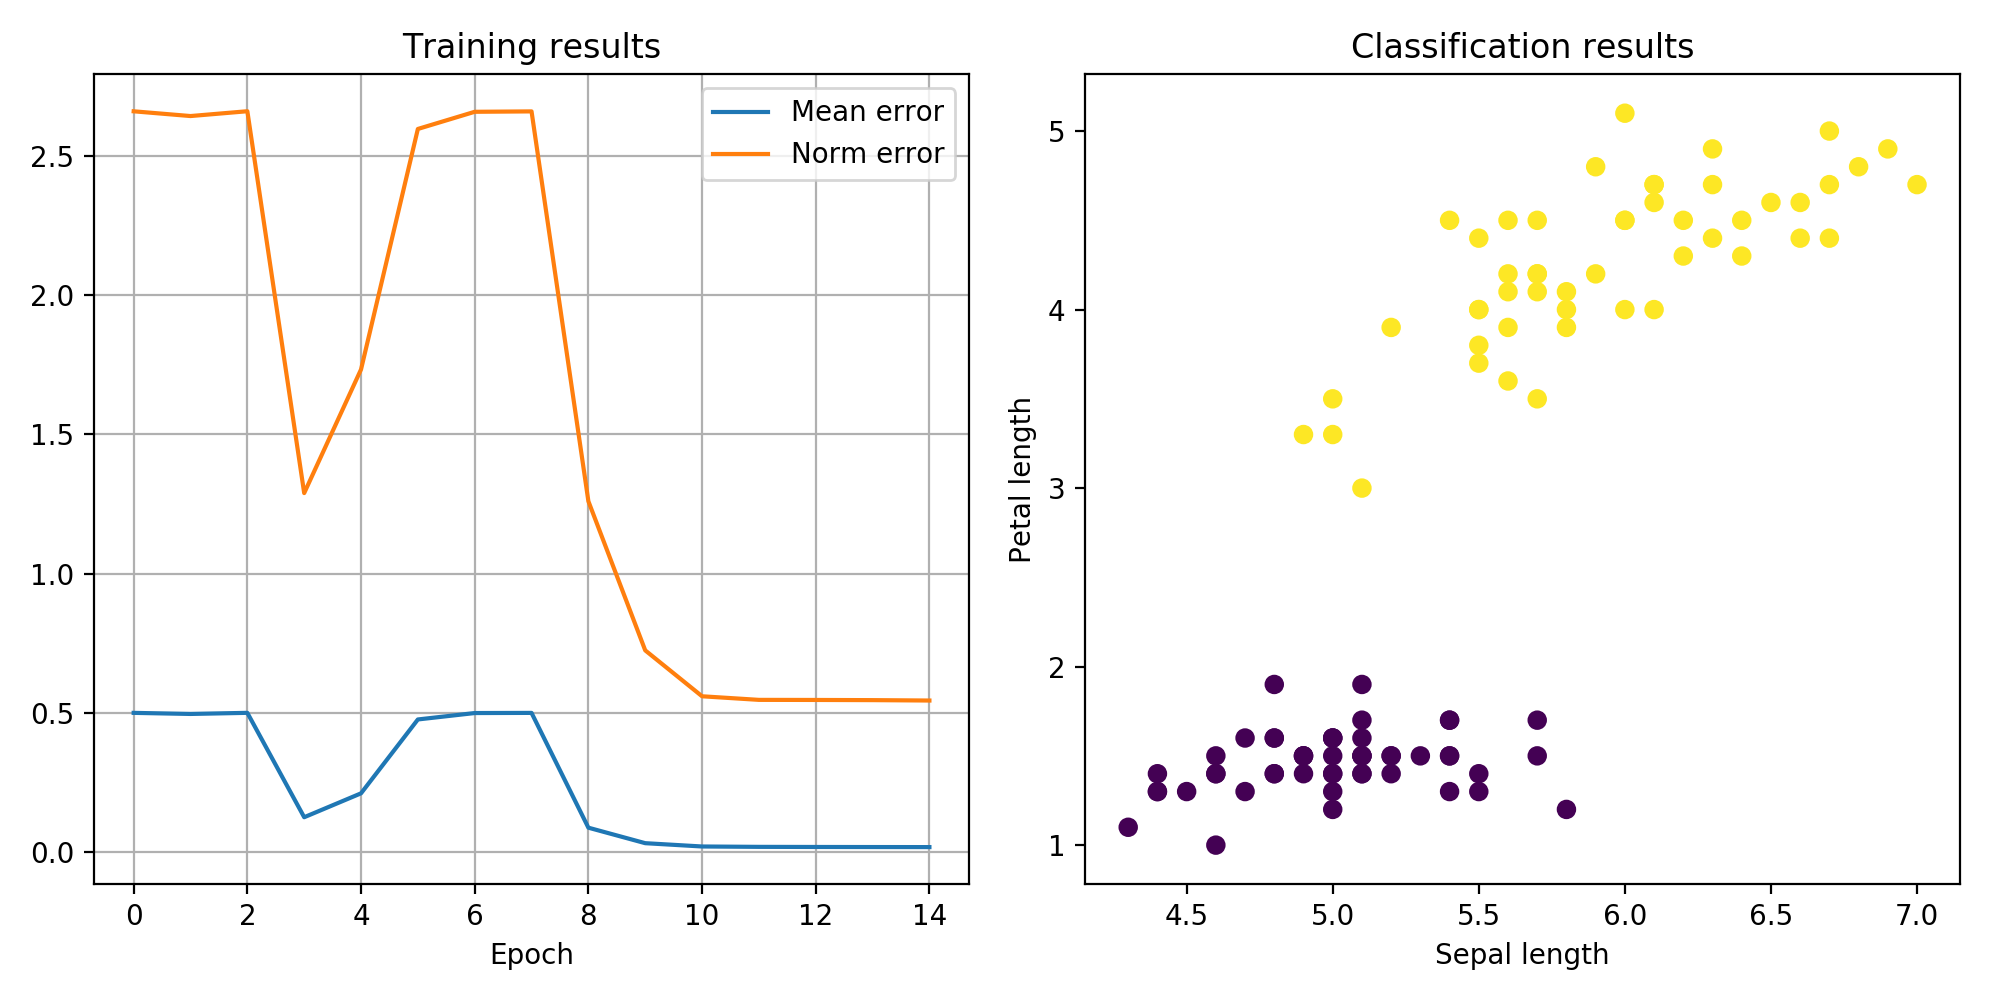
\includegraphics[scale=0.47]{LogisticRegressionIris.png}

In the left diagram, we have plotted the norm and the mean of the error vector after a given number of epochs. We see that the network converges already after a few epochs, and the average error becomes very small. The norm of the error vector, however, is always different from zero
as the $p_i$ are never exactly $1$ or $0$. Instead, when asking the network to classify a sample, we assign the sample to class $1$ if $p > 0.5$ and to class $0$ otherwise. On the right hand side, the result is displayed. Each item represents one sample with its features sepal length and petal length. The color indicates the class to which the sample has been assigned after the training has been completed. We see that the logistic regression model is able to correctly detect the two clusters which can obviously be linearly separated.

Obviously, logistic regression performes less satisfactory if the underlying distribution does not allow a clear separation of the training set into two classes. In the following example, a training set of 500 samples has been created which consists of data points two clusters, both following a standard
normal distribution in two dimensions with covariance matrix
$$
\begin{pmatrix}
0,7 & 0 \\
0 & 0,7
\end{pmatrix}
$$
with mean values $(6.5, 4.5)$ and $(5. 1.5)$, and the samples have been labeled according to the cluster from which they have been sampled.

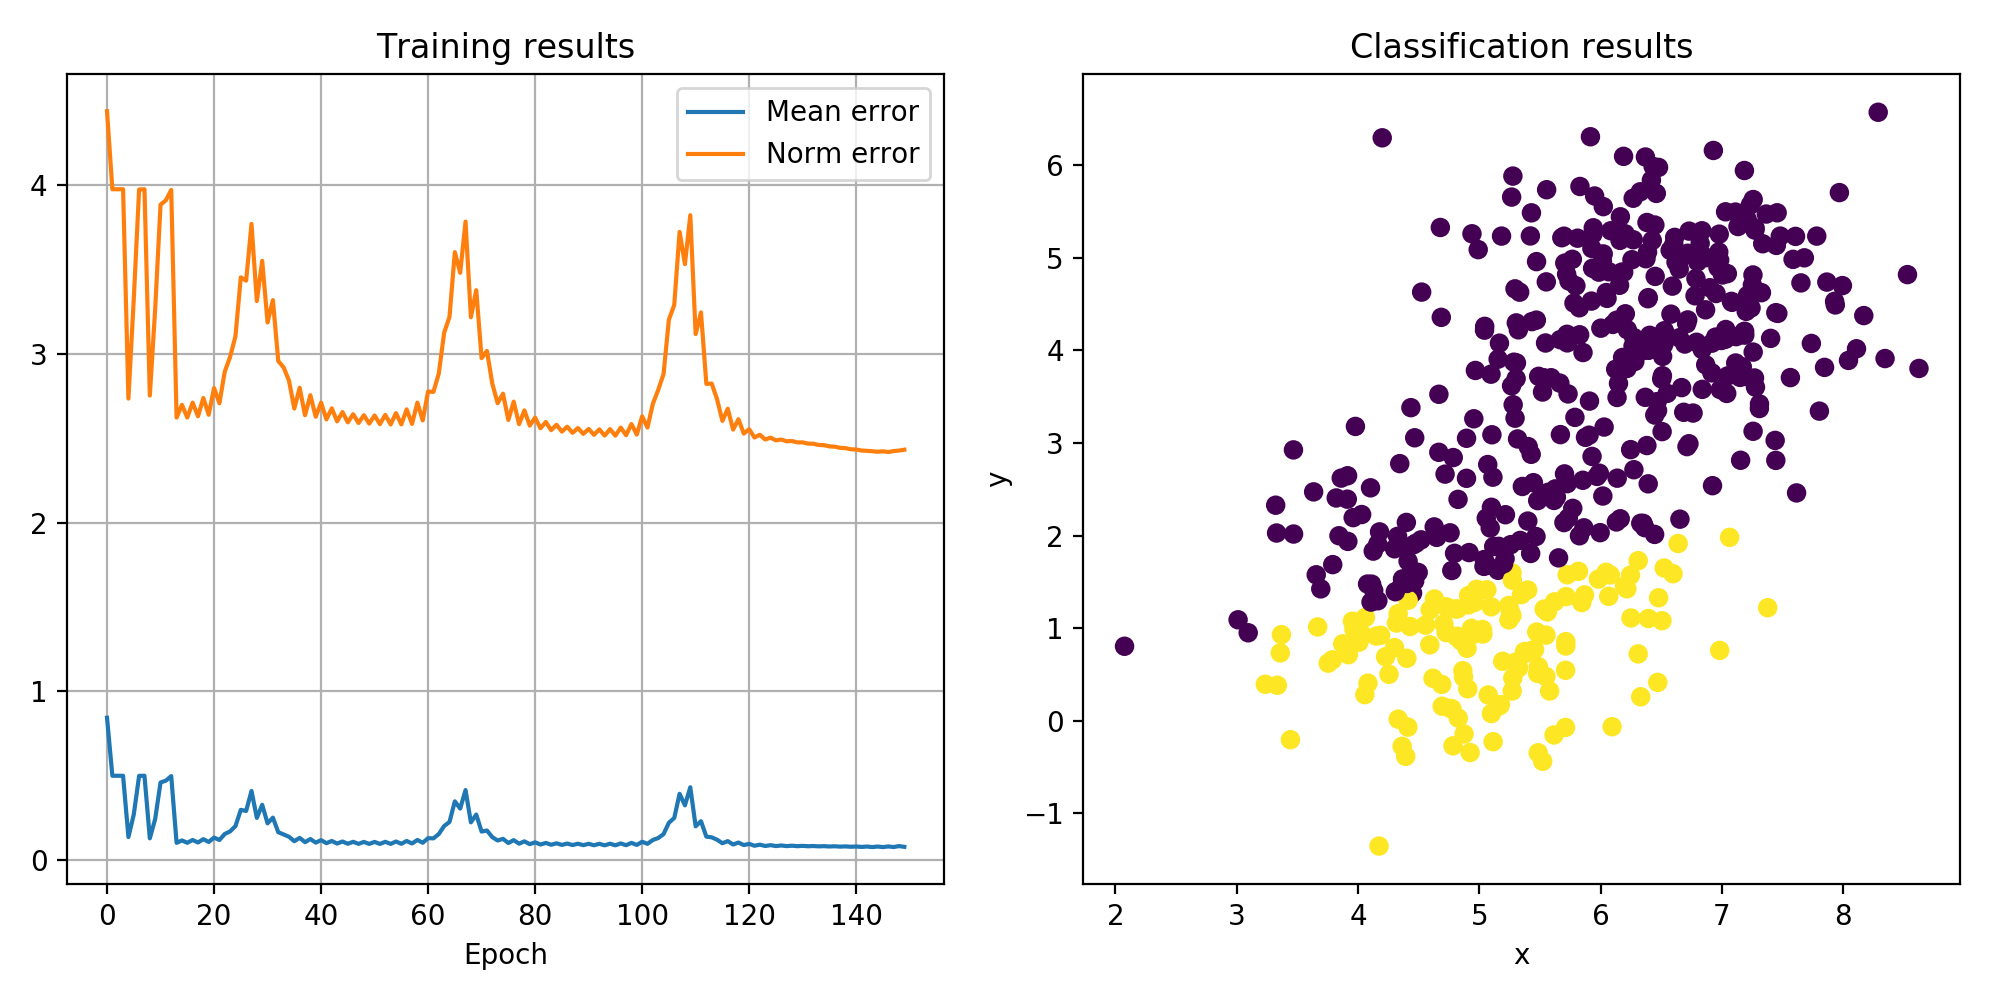
\includegraphics[scale=0.47]{LogisticRegressionSample.png}

As we can see in the picture on the right hand side, these clusters overlap significantly. The model is trying to separate the clusters along the line where blue and yellow cluster points overlap, but - as we can see from the metrics on the right hand side - the errors oscillate and the network does not converge. In fact, there are even phases where the error goes up again for a few epochs. 

\chapter{Entropy and Kullback-Leibler divergence}\label{sec:entropy-and-kullback-leibler-diverergence}

Let us now relate this statistical model to a simple neuronal network with a sigmoidal activation function. Specifically, consider a neuronal network with one input layer consisting of $d$ units and an output layer consisting of one unit only. If we denote the activations of the units in the input layer by $x_i$, the activation of the output unit is given by 
$$
z = \sum_i w_i x_i = w^t x
$$
with a weight vector $w \in \R^d$. We then apply the sigmoid function as an activation function, i.e. the output of the unit is
$$
\sigma(z) = \frac{1}{1+e^{-z}}
$$

This is already very close to our logistic regression model discussed in the last section. A given activation of the input units is a $d$-dimensional vector which is a point $x^i$ in a sample, and we can identify the resulting output of the network as 
$$
P(Y = 1 | X = x)
$$ 
in the regression model. We can now understand why such a network is used as a binary classifier. The inputs represent features of a sample - in our initial example, this would be the features of being able to fly and the bodylength - and the output approximates the probability that the object at hand belongs to a certain class, birds in our example. During training, the weights are adapted such that the output comes as close to the actual distribution $Y$ as possible, so that when we apply the network to a new object which has not been part of the sample, the output is still a good approximation to the value of $Y$ on this sample points. 

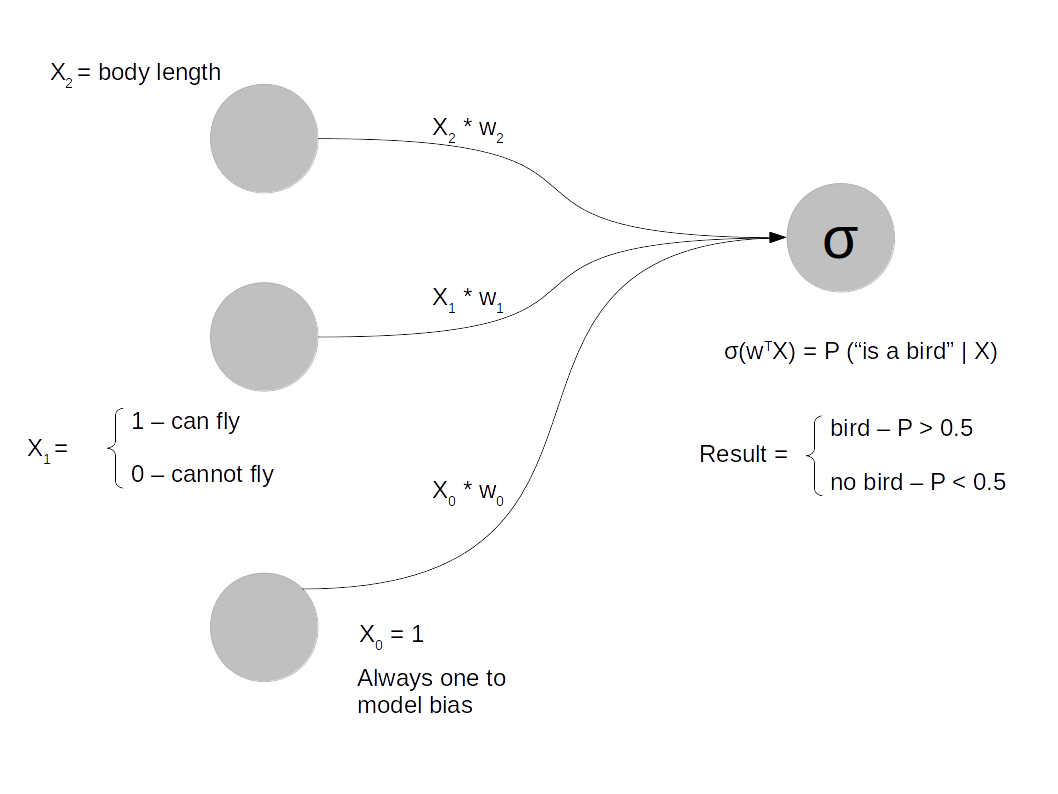
\includegraphics[scale=.4]{BirdClassifier.png}

But how do we train the model? Typically a neuronal network is trained by defining a loss function $l$ which depends on the weigths $w$ and the {\em labels}, i.e. the given sample $y^i$, and iteratively adjusts the weights using a method like gradient descent to minimize the loss function. A very often used loss function is the {\em cross entropy}, and we will now study how the cross entropy is defined and why the resulting loss function is actually nothing else than minus the logarithmic likelihood function from our logistic regression model.

Let us first recall a few definitions. To avoid some technicalities, we will restrict ourselves to the case of discrete random variables, which is not a real restriction in the applications to neural networks as any quantity calculated by a machine with finite word length has a finite and therefore discrete range. We refer the reader to standard textbooks in statistics and probability theory for more details, for instance \cite{Schervish}, section 2.3.2 or \cite{LehmannRomano}, section 11.2. The first definition that we will need is the Kullback Leibler divergence. So let us assume that we are given two random variables $X$ and $X'$ with the same range ${\mathcal X}$, described by probability mass functions
$$
f(x) = P(X = x)
$$
and
$$
f'(x) = P(X' = x)
$$
\begin{defn}
We define the Kullback-Leibler divergence or relative entropy $D_{KL}(X,X')$ as the expectation of the logarithmic difference of $f$ and $f'$, where the expectation is taken with respect to the distribution of $X$, i.e.
$$
D_{KL}(X, X') = \sum_{x \in {\mathcal X}} f(x) \ln \frac{f(x)}{f'(x)}) = {\mathbb{E}}_{P(X)} \ln \frac{P(X = x)}{P(X' = x)}
$$
\end{defn}
This definition assumes that $f'$ is absolutely continous with respect to $f'$, i.e. that $f'(x)=0$ implies $f(x)=0$, so that the corresponding summand is zero. There is also a conditional version of this definition which is as follows.
\begin{defn}
Suppose that $X$ and $X'$ are random variables. We then define the conditional Kullback-Leibler divergence of $X$ and $X'$ given a third discrete random variable $T$ to be 
$$
D_{KL}(X, X' | T) = \sum_{t} P(T=t) \sum_{x \in {\mathcal X}} P(X = x  | T = t) \ln \frac{P(X = x | T = t)}{P(X' = x | T = t)}
$$
\end{defn}
Note that this is actually an expectation value - for each value $t$, we determine the Kullback-Leibler divergence between $X$ conditioned on $T = t$ and $X'$ conditioned on $T = T$, and then we take the average over all values of $t$, i.e. the expectation value.  Observing that 
$$
P(X = x | T = t) P(T = t) = P(T = t, X = x)
$$
this can also be written as the expectation value
$$
\sum_{x,t} P(X = x, T = t) \ln \frac{P(X = x | T = t)}{P(X' = x | T = t)} = \mathbb{E}_{P(T,X)} \ln \frac{p_{X}(x|t}{p_{X'}(x | t)}
$$
where we denote by $p_X(\cdot | t)$ the probability mass function for $X$ conditioned on $T = t$, similarly for $X'$, and by $P(T,X)$ the joint probability distribution of $T$ and $X$. 
This in turn is the same as
$$
\sum_{x,t} P(X = x, T = t) \ln \frac{P(X = x , T = t)}{P(X' = x , T = t)} = \mathbb{E}_{P(T,X)} \ln \frac{p_{(X,T)}(x,t)}{p_{(X',T)}(x,t)}
$$
In other words, the conditional Kullback-Leibler divergence between $X$ and $X'$ conditioned on $T$ is the same as the Kullback-Leibler divergence between the joint distributions $(X,T)$ and $(X',T)$. This is only true because the distribution $T$ on which we condition is the same on both sides, in a more general setting with two different distributions $T$ and $T'$, we would get an additional term $D_{KL}(T,T')$, a fact which is known as the chain rule for relative entropy.

It is well known that the Kullback-Leibler divergence between two probability distributions is always non-negative and is zero if and only if the two distributions agree almost surely. Thus, in a certain sense, the Kullback-Leibler divergence is a measure for the distance of two distributions in an abstract space of all probability distributions. Note, however, that this is not a real metric, as it is not symmetric.

We will know investigate a second quantity, called the {\em cross entropy}, which is often used to express the distance between two probability distributions, and investigate how it relates to the Kullback-Leibler divergence. Recall that for a discrete random variable $X$ taking values in some finite set $\mathcal X$, we define the {\em entropy} of $X$ to be
$$
H(X) = {\mathbb{E}}_{P(X)} \ln \frac{1}{P(X = x)} = - \sum_x P(X = x) \ln P(X = x)
$$
This quantity was introduced in \cite{Shannon}, which is considered to be the starting point of modern information theory. In this paper, Shannon argues that up to a constant, the entropy is the only measure of the uncertainty that we have about the outcome of a random event that fulfills certain reasonable assumptions. For instance, $H(X) \geq 0$ and $H(X) = 0$ only if $X$ is atomic, i.e. $P(X = x) = 1$ for some $x \in {\mathcal X}$. In addition, the entropy is maximized by a uniform distribution for which all outcomes have the same probability. This is in accordance with our
intuition that the uniform distribution is the distribution with the lowest information gain. 

The entropy is additive, i.e. if $X$ and $Y$ are discrete and independent random variables and $U=(X,Y)$ the joint distribution, we have
$$
H(U) = H(X) + H(Y)
$$
Thus if we observe two independent events, the information we gain from observing $X$ and $Y$ is the sum of the information that we gain from $X$ and $Y$ alone.

Again, there is a conditional version of entropy. The idea is the same as for the Kullback-Leibler divergence - we determine the entropy for each of the conditional distributions and then average over the values of the random variable on which we condition. Thus we get the following

\begin{defn}
Suppose that $X$ and $T$ are discrete random variables. We define the conditional entropy of $X$ conditioned in $T$ to be
$$
H(X | T) = - \sum_t P(T = t)  \sum_x P(X = x | T = t) \ln P(X = x | T = t) 
$$
\end{defn}

Note that using $P(X = x | T = t) P(T=t) = P(X = X, T = t)$, we can write the conditional entropy equally well as
$$
H(X | T) = - \mathbb{E}_{P(X,T)} \ln P(X = x | T = t)
$$
where $P(X,T)$ denotes the joint distribution of $X$ and $T$. It is also straightforward to show that
$$
H(U) = H(X | Y) + H(Y)
$$
where again $U = (X,Y)$ is the joint distribution of $X$ and $Y$. Thus the conditional entropy given $Y$ measures how much information we gain from observing $X$ after already having observed $Y$. Combining this with our earlier result on the entropy of a joint distribution, we see in particular that $H(X | Y) = H(X)$ if $X$ and $Y$ are independent.

Let us now investigate how the Kullback-Leibler divergence is related to the entropy. So suppose that we are given two discrete random variables $X$ and $Y$ described by probality mass functions $p_X$ and $p_Y$. Then the Kullback-Leibler divergence is
$$
D_{KL}(X,Y) = \sum_a p_X(a) \ln \frac{p_X(a)}{p_Y(a)}
$$
Obviously, this can be written as
$$
D_{KL}(X,Y) = \sum_a p_X(a) \ln p_X(a) - \sum_a p_X(a) \ln p_Y(a)
$$
The first term is easily recognized as $-H(X)$. Thus
$$
D_{KL}(X,Y) + H(X) = - \sum_a p_X(a) \ln p_Y(a)
$$
This quantity is called the {\em cross entropy} between $X$ and $Y$. 

\begin{defn}
Suppose that $X$ and $Y$ are discrete random variables with a common range ${\mathcal A}$. Then we call the quantity
$$
H(X,Y) = - \sum_{a \in {\mathcal A}} P(X = a) \ln P(Y = a)
$$
the cross entropy between $X$ and $Y$. 
\end{defn}

We have claimed above that the cross entropy is another measure for the distance between $X$ and $Y$. In fact, we have seen above that
$$
H(X,Y) = H(X) + D_{KL}(X,Y)
$$
Thus for a fixed random variable $X$, the Kullback-Leibler divergence and the cross entropy differ only by a constant term, namely the entropy of $X$. Thus they both measure to what extent $Y$ differs from $X$. Of course, we can also replace the Kullback-Leibler divergence and the entropy by their conditional versions to obtain a {\em conditional cross entropy}.

After these preparations, let us now come back to the logistic regression model and try to understand the relation between Kullback-Leibler divergence, loss function and cross entropy. In fact, we will study a slightly more general model. We assume that $X^i$ and $Y^i$ are discrete random variables, with $X^i$ taking values in some subset ${\mathcal X}$ of $\R^d$ and $Y^i$ taking values in some subset ${\mathcal Y} \subset \R^s$, where $i$ ranges from $1$ to the sample size $N$. We let 
$$
U^i  = (X^i,Y^i)
$$
denote the combined random variables taking values in $\R^{d+s}$ and assume that the $U^i$ are independent and identically distributed. Further, we let $X = (X^1, X^2, \dots, X^N)$ be the random variable with values in $\R^{Nd}$ obtained by combining the $X^i$ into a single variable,
and similarly for $Y$ and $U$.

Recall that if $X$ and $Y$ are independent, then $f(X)$ and $g(Y)$ are independent for any two measurable functions $f$ and $g$. Applying this to projections, we see that the $X^i$ are mutually independent and similarly the $Y^i$ are mutually independent. We do, however, not assume
that $X^i$ and $Y^i$ are independent. Instead, we assume a relationship
$$
P(Y^i = y | X^i = x) = f(x,y ; \Theta_0)
$$
for a function $f$ depending on $u = (x,y)$ which is parametrizable via a parameter $\Theta$. 

In the case of logistic regression, we have ${\mathcal Y} = \{0,1\}$ and the function $f$ is given by
$$
f(x,y; \Theta) = y^p (1-y)^{1-p}
$$
with $p = p(x; \Theta) = \sigma(\Theta^t x)$. However, our model is more general and can in general model a neuronal network with $d$ input units and $s$ output units, when we allow more general functions $f$ and $\Theta$ represents the weights of the neural network. The sample $U^i$ is then a model for the training set, which we assume to be drawn from the distribution corresponding to some parameter $\Theta_0$, and during training, we try to iteratively determine $\Theta$ to be as close to $\Theta_0$ as possible. 

Let us now try to write down the likelihood function in this model. So suppose that $u^1, \dots, u^n$ is a realization of the $U^i$, i.e. a given actual sample, which we write again as $u^i = (x^i y^i)$. The $y^i$ are the labels and the $x^i$ the features of the i-th point in the sample. The full sample is then represented by vectors $y$ and $x$ and the conditional likelihood of $\Theta$ given the input data is given by
\begin{align*}
L(\Theta) = P(Y =y | X = x ; \Theta) &= \frac{P(U = u)}{P(X =x)} \\
&= \frac{\prod_i P(U^i = u^i)}{\prod_i P(X^i = x^i)} \\ 
&= \prod_i \frac{P(U^i = u^i)}{P(X^i = x^i)} \\
&= \prod_i P(Y^i = y^i | X^i = x^i) = \prod_i f(x^i,y^i;\Theta)
\end{align*}
Maximizing the likelihood therefore amounts to minimizing the {\em loss function}
$$
l(\Theta) = - \frac{1}{N} \ln L(\Theta) = - \frac{1}{N} \sum_i \ln f(x^i,y^i ; \Theta)  
$$
where the reason for the factor $N$ will become clear soon. Now we can define random variables $F_i$ by
$$
F_i = \ln f(X^i, Y^i ; \Theta) = f(U^i ; \Theta)
$$
As the $U_i$ are assumed to be independent and identically distributed, the same is true for the $F_i$. We can therefore apply the law of large numbers to conclude that 
\begin{align}\label{eq:expectationvaluelossdistribution}
\lim_{N \rightarrow \infty} l(\Theta) = - {\mathbb{E}_{P(U;\Theta_0)}} \ln f(u;\Theta) 
\end{align}
where $P(U;\Theta_0)$ denotes the probability distribution from which the sample $U^i$ was drawn, i.e. the real distribution corresponding to the real parameter $\Theta_0$. But this expectation value can be written as
\begin{align*}
- {\mathbb{E}_{P(U;\Theta_0)}} \ln f(u;\Theta)  &=  {\mathbb{E}_{P(U;\Theta_0)}} \ln \frac{1}{ f(u;\Theta)} \\
&=  {\mathbb{E}_{P(U;\Theta_0)}} \ln  \frac{f(u;\Theta_0)}{f(u;\Theta)} - {\mathbb{E}_{P(U;\Theta_0)}} \ln f(u;\Theta_0)
\end{align*}
The first term is easily identified as the conditional Kullback-Leibler divergence between the distributions of $Y$ given $X$ belonging to the parameters $\Theta_0$ and $\Theta$. The second term is the conditional entropy of the distribution belonging to the parameter $\Theta_0$. Thus we have found that {\em for a sufficiently large sample, the negative log likelihood function is - up to a constant - approximately equal to the conditional cross entropy between the real distribution from which the sample was drawn and the distribution given by $\Theta$.  Therefore minimizing the cross entropy is essentially the same as maximizing the conditional likelihood. }

Thus we have reconciled the approach to the logistic regression model via a maximum likelihood estimator with the approach that is typically presented in introductions to neuronal networks and based on the principle of minimizing the cross-entropy - the outcome will be the same. Popular software packages for working with neuronal networks like Theano (\cite{Theano} or TensorFlow (\cite{Tensorflow}) do offer support to calculate the cross entropy for a logistic distribution and also support automatic differentiation to calculate gradients, so that a gradient descent approach can be applied to iteratively determine a mimimum of the loss function - and this is exactly what happens during the training phase of a neuronal network.

There is another interpretation of the maximum likelihood estimator in terms of cross entropy which is worth mentioning. So far we have tried to minimize the distance between the distribution corresponding to $\Theta$ from the real distribution which we implicitly did assume to be given by some parameter $\Theta_0$. What happens if we drop this assumption? We then need to measure the distance to some other distribution that we consider as being the ``real'' distribution from which the $Y^i$ are sampled. An obvious candidate for this is the distribution which explains the observed sample exactly, i.e. the {\em empirical distribution} which assigns to each vector $u$ the average number of times this vector is observed. For this distribution, the expectation value of any measurable function is the average over the observed values. In particular, if we replace $P(U,\Theta_0)$ in equation \eqref{eq:expectationvaluelossdistribution} by the empirical distribution, the limit turns into an equality. Thus we see that the loss function can alternatively be interpreted as the conditional cross entropy between the empirical distribution based on the observed sample and the distribution given by the parameter $\Theta$. 

\chapter{Multinomial logistic regression}

So far we have studied the logistic linear regression model, understood why this model describes a simple neuronal network acting as a classifier and studied the loss function that is typically used to train such a network. The logistic regression model we have used so far is, however, restricted to a dependent variable $Y$ which only takes on two values, i.e. a binary random variable.  Let us now assume that we want to model the conditional probability for an outcome variable $Y$ which can take on $K$ distinct values, for simplicity this could be $\{1, \dots, K\}$. Thus, instead of generating one probability $p_i$ from each sample $X^i$, we now have to create $K$ distinct probabilities $p^i_k$ that add up to one for a fixed $i$. A standard choice for this purpose is the {\em softmax function} which is a function that maps $\R^K$ to itself and is given by 
$$
s_j(z_1, \dots, z_K) = \frac{e^{z_j}}{\sum_{i=1}^K e^{z_i}}
$$
There is an obvious relation to the sigmoid function. In fact, for $K=2$, we have
$$
s_1 (z_1, z_2) = \sigma(z_1 - z_2)
$$
Obviously
$$
\sum_k s_k(z_1, \dots, z_) = 1
$$
so that the softmax function is well suited to modelling probabilities that add up to one.  In order to build an equivalent for the logistic regression model, we now choose our weights to be a matrix $W$ with $d$ rows and $K$ columns, where again $d$ is the number of features, i.e
$X^i \in \R^d$. Similarly, we combine all feature vectors $X^i$ into a matrix with $N$ rows and $d$ columns. We can then form the matrix $X \cdot W$ which has $N$ rows and $K$ columns. Each of the rows of this matrix - which we denote by $(X \cdot W)^i$ - is then a $K$-dimensional vector which is given by
$$
((X \cdot W)^i_j = \sum_{k=1}^d X^i_k W^k_j
$$
and 
$$
p^i_j = P(Y^i = j | X^i = x^i) = s_j((X \cdot W)^i)
$$
which can be written in an even more compact form as
$$
p = s(X \cdot W)
$$
Then the i-th row of this matrix will represent the $j = 1, \dots, K$ probabilities for $Y^i$ to take value $j$.  

Let us now again calculate the likelihood function, the resulting loss function and its gradient. For calculations, especially those that involve logarithms, it is more convenient to use a {\em 1-of-K encoding}. Specifically, we define a random variable $T$ which takes values in $\R^K$ with the restriction that each component can only be one or zero and that there is always exactly one component which is one. We relate $T$ to $Y$ by the prescription that the j-th component of $T$ is one if and only if $Y=j$. In other words
$$
P(T^i_j = 1  | Y^i = y^i) = p^i_j 
$$
This has the advantage that for a given target vector $t$, we can write
$$
P(T^i = t^i | Y^i = y^i) = \prod_j {p^i_j}^{t^i_j} 
$$
where of course only one of the products will be different from one as only one of the $t^i_j$ is different from zero. This makes it easy to write down the loss function, again remembering that the $Y^i$ and thus the $T^i$ are supposed to be independent:
$$
l(W) = - \ln L(W) = - \sum_{i,j} t^i_j \ln p^i_j
$$
Now let us again calculate gradients. First, a short calculation shows that
$$
\frac{\partial s_i}{\partial z_j} =  s_i s_j + \delta_{ij} s_j
$$
where as usual $\delta_{ij}$ is the Kronecker-Delta. If we denote the activation by
$$
a^i_j = \sum_{k=1}^d X^i_k W^k_j
$$
then we have
$$
\frac{\partial a^i_j}{\partial W^s_t} = \delta_{jt} X^i_s
$$
and
$$
p^i_j = s_j (a^i)
$$
Therefore the chain rule gives us
\begin{align*}
\frac{\partial p^i_j}{\partial W^s_t} &= \sum_k \frac{\partial p^i_j}{\partial a^i_k} \frac{a^i_j}{\partial W^s_t}   
=\frac{\partial s_j}{\partial a^i_t} X^i_s \\
&= (-s_j s_t  + \delta{tj} s_j) X^i_s \\
&= (-p^i_j p^i_t + \delta_{tj} p^i_j) X^i_s
\end{align*}
and therefore
$$
\frac{\partial}{\partial W^s_t} \ln p^i_j = (-p^i_t + \delta_{tj})X^i_s
$$
We can use this result to calculate the derivative of the loss function and obtain
$$
\frac{\partial l}{\partial W^s_t} = \sum_i (t^i_t + \sum_j t^i_j p^i_t) X^i_s = \sum_i (p^i_t - t^i_t) X^i_s
$$
where we have used that $\sum_j t^i_j = 1$. Again this can be interpreted as the observation $X$ times an error term that measures the difference between the target $t$ and the actual result $p$. If we define a matrix $E$ as
$$
E = T - p
$$ 
we can write this as
$$
\frac{ \partial l}{\partial W^s_t} = - (X^t E)^s_t
$$
and we obtain the following rule to update our weight vectors in each iteration:
$$
W \leftarrow W + \lambda (X^t E)
$$
where again $\lambda$ denotes the step size in the gradient descent algorithm. Thus it is again very easy to implement multinomial regression in a programming language like Python:

\begin{lstlisting}[frame=single,language=Python,caption=Implementation of the training phase in Python]
for step in range(epochs):
    # 
    # The activation is  given by the matrix product X W 
    #
    p = softmax(np.matmul(X, W))
    # 
    # Next we compute the error
    E = target - p
    #
    # finally we update the weights
    #
    W = W + learning_rate * np.matmul(np.transpose(X), E)
\end{lstlisting}

Note that this algorithm assumes that the target is given by a sample of the random variable $T$, i.e. in the 1-of-K encoding. The result of the algorithm is then described by the value of $p$ for a test sample, and the value in column $j$ and row $i$ of $p$ is the probability that the sample $i$ belong to class $j$.  

Again, we can use the iris data set as an example. In this case, we have four features (sepal length, petal length, sepal width, petal width), so that $d=4$, and three classes corresponding to the three types of flowers, i.e. $K=3$. This corresponds to a network with four input units and three output units. The following diagram shows the result of training such a network for 300 epochs, using again a learning rate of 0.01. Again, the left hand side displays the learning progress, measured in terms of norm and mean of the absolute value of the error vector, whereas the right hand side visualizes the classification results in a 3-dimensional scatter plot, where we have suppressed one of the four features.

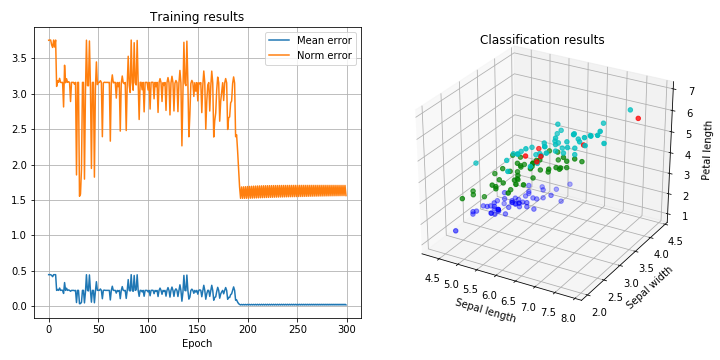
\includegraphics[scale=0.47]{MultinomialRegressionIris.png}

In the plot on the right hand side, samples which are not correctly classified are displayed in red. Even after a few hundred epochs, we still have between 3 and 6 incorrectly classified samples, We see that these are sample points that are hidden in cluster of samples of a different species, and a linear classifier is no longer able to clearly separate these points from their closest neighbor. So our simple model is reaching its limit.

It is instructive to see how the learning algorithm changes if we replace our multinomial regression model by a model with $K$ independent output variables $Y_j$. In a multinomial model, the targets $T_j$ are obviously not independent, as only one of them can be one. In a model with $K$ independent binary variables $Y_j$, each variable can be $0$ or $1$ and the variables are fully independent. We can model this using again the logistic regression function instead of the softmax function, i.e. we assume that our conditional probabilities are given by
$$
P(Y^i_j = 1 | X^i = x^i) = p^i_j = \sigma((XW)^i_j) = \sigma(\sum_k X^i_k W^k_j)
$$
where again $X$ is a matrix with $N$ rows (the size of the sample) and $d$ columns (the number of features), and $W$ is a matrix with $d$ rows and $K$ columns, and that the $Y_j$ are independent. Then our loss function is
$$
l(W) = - \ln L(W) = - \sum_{i,j} ( y^i_j \ln(p^i_j) +  (1 - y^i_j) \ln (1-p^i_j))
$$
Using a calculation similar to the one before, we find that
$$
\frac{\partial p^i_j}{\partial W^s_t} = p^i_j (1-p^i_j) \delta_{jt} X^i_s
$$
and
$$
\frac{\partial l}{\partial W^s_t} = - \sum_i X^i_j (y^i_t - p^i_t)
$$
Thus, if we again define an error matrix as
$$
E = Y - p
$$
we have
$$
\frac{\partial l}{\partial W^s_t} = - (X^T E)^s_t
$$
In other words, the rule to update the weights for a model with $K$ independent binary output variables has exactly the same form as the update rule for the weights in the multinomial model (but of course the rule to calculate the matrix $p$ and thus $E$ is different, using $\sigma$ instead of a softmax function). It is worth mentioning that this is not just pure coincidende, but true for a larger class of models, so called general linear models (see \cite{Bishop}, secton 4.3.6).

So when do we use a softmax activation function and when do we use a sigmoid activation function when designing a neuronal network? The answer depends (surprise) on what you want to model. If the purpose is a classification where the different classes are mutually disjoint, then a multinomial model and correspondingly a softmax activation function is more appropriate. If, however, we want to model independent binary variables, a sigmoid function is the better choice. In practice, hidden layers of neuronal networks tend to use a sigmoid activation (or an alternative choice like a rectified linear unit activation function (RELU ) whereas the final output layer is often modelled using a softmax activation function. 

\chapter{Feed forward networks and backpropagation}

So far we have considered statistical models that are described by a conditional probability distribution of the form
$$
P (Y^i| X^i ) = h(XW)
$$
with a matrix $X$ describing the inputs to the model, a matrix `$W$ describing weights and bias and a function $h$ which was either the sigmoid function or the softmax function. We have used these models as linear classifiers. The output for the i-th feature vector in the sample is then given by multiplying the matrix $W$ of weights with the i-th row of $X$, i.e. the input to the activation function is linear in the feature vector. Thus, feature vectors that only differ by an element in the kernel of $W$ will yield the same output. This implies that if we use these models as classifiers, they will only be able to distinguish different sets of feature vectors that can be separated by linear submanifolds in the sample space.

In order to obtain more general models, we can start to implement more complex networks which have layers. A {\em layered neuronal network} consists of a set of layer $0, 1, 2, \cdots$ of neurons (usually called {\em units} for short) such that a unit in layer $i$ receives input only from units in layer $i-1$, and each layer acts as a simple linear classification model as discussed above.

To make this more precise, suppose we are again given a matrix $X$ of random variables with $N$ rows and $d$ columns, where $N$ is interpreted as the sample size and $d$ as the number of features. Suppose further that we are given a set of matrices $W^i, i = 1, \cdots, L$. We will denote the element at row $s$ and column $t$ of matrix $i$ by $W^{i,s}_t$.  We can then form the matrix
$$
Z^1 = \sigma(X W^1) 
$$
to form a logistic regression model. We can then feed the output of this model as input into a second logistic regression model, i.e. we consider
$$
Z^2 = \sigma(Z^1 W^2)
$$
and so forth. The output of the last layer is given by 
$$
Z^L = s(Z^{L-1} W^L) )
$$
i.e. we use the softmax function as activation layer (other choices are possible and must of what follows applies to other activation functions as well). We call the quantity
$$
a^i = Z^{i-1} W^i
$$
the {\em activation} of layer $i$ for $i > 0$. Thus $a^{k,i}_s$ denotes the activation of unit $s$ in layer $i$ for sample $k$. Moreover, we set $X=Z^0$. The situation is illustrated below, where not all connections are shown.

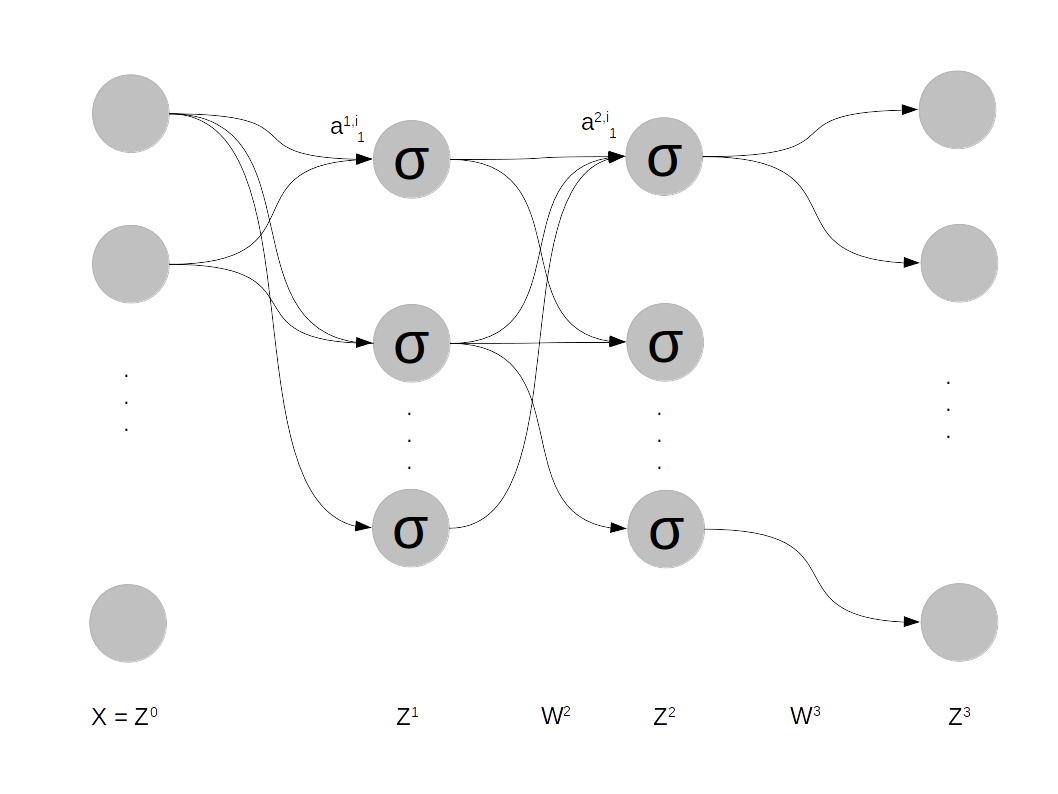
\includegraphics[scale=0.42]{LayeredNetworkTopology.png}

The last layer $Z^L$ is usually called the {\em output layer}. The first layer $Z^0$ is called the {\em input layer}. All other layers are called {\em hidden layers}. Thus our example is a network with one softmax output layer, two sigmoid hidden layers and one input layer. By convention, the weight matrix $W^i$ connects layer $i-1$ and layer $i$. Note that the number of rows of the matrix $W^i$ is the number of units in the layer $i-1$, and the number of columns is the number of units in layer $i$. 

Again we interpret the model as calculating a probability distribution, i.e. we define a distribution conditional on $X$ by
$$
P(Y^i = j | X^i ) = Z^{L,i}
$$
and assume that the $X^i$ and the $Y^i$ are independent. Our goal will again be to apply the maximum likelihood method to fit all weights $W^i$ to a given labeled sample of feature vectors, where we assume that the labels are given by a matrix $T$ where each row is the labeling of the corresponding sample in a 1-of-K encoding. In order to determine the maximum of the likelihood function, we again intend to use the method of gradient descent. Using the results of the previous section on the multinomial regression model, we can immediately write down the loss function:
$$
l(w) = - \sum_{i,j} T^i_j \ln Z^{L,i}_j = - \sum_{i,j} T^i_j \ln s_j (a^{L,i}) 
$$
However, this is a significantly more complex function of the weights than in the case of one layer, so we need a clever way to organize the calculation to be able to run it efficiently. The standard method for that purpose is known as the {\em backpropagation algorithm} (see \cite{RHW}), which we now explain. We start by computing the partial derivatives of the loss function with respect to the activation of the last layer. Thus we compute
\begin{align*}
\frac{\partial}{\partial a^{L,s}_t} \ln s_j(a^{L,i}) = \frac{1}{s_j} \delta_{is} (-s_i s_j + \delta_{jt} s_j) = \delta_{ij} (\delta_{jt} - s_t)
\end{align*}
and obtain
\begin{align*}
\frac{\partial l}{\partial a^{L,s}_t} &= - \sum_{i,j} T^i_j \delta_{ij} (\delta_{jt} - s_t) \\
&= - T^s_t + \sum_j s_t T^s_j = - T^s_t + s_t \sum_j T^s_j = - T^s_t + Z^s_t
\end{align*}
Thus this derivative is given by the error term that we already met before, which is imply the difference between the actual output ($Z^s_t$) and the target ($T^s_t$) and which we have now identified as a partial derivative. This motivates the definition of an error term for the deeper layers. We call
$$
E^{i,s}_t = - \frac{\partial l}{\partial a^{i,s}_t}
$$
the error term for layer $i$. Then our calculation shows that the error for the output layer is
$$
E^L = T - Z^L 
$$
as we expect. Before we turn to the question how we can compute the error terms for the other layers, let us first try to understand why these terms are useful. Suppose we wanted to calculate the derivative of the loss function with respect to a weight matrix element $W^{i,s}_t$ in the weight matrix that determines the input to layer $i$. The loss function can be written as a function of the weights of all layers $j > i$ and the input to layer $i$. Thus the dependency on the weights for layer $i$ can be written as an implicit dependency via the inputs to layer $i$, i.e. the activation of layer $i$. Using the chain rule, this implies that
$$
\frac{\partial l}{\partial W^{i,s}_t} = \sum_{p,q} \frac{\partial l}{\partial a^{i,p}_q} \frac{\partial a^{i,p}_q}{\partial W^{i,s}_t} 
$$
The first term in each summand is simply minus one times the error term that we have defined above. The second term, however, is easy to calculate, because the activations are simply given by the matrix product of input and weights, so its derivatives with respect to the weights are simply the elements
of the input matrix:
$$
\frac{\partial a^{i,p}_q}{\partial W^{i,s}_t}  = \frac{\partial}{\partial W^{i,s}_t} (Z^{i-1} W^i)^p_q = \delta_{tq} Z^{i-1,p}_s
$$
We therefore obtain
$$
\frac{\partial l}{\partial W^{i,s}_t} = - \sum_p  E^{i,p}_t Z^{i-1,p}_j = - ((Z^{i-1})^T E^i)^s_t
$$
Thus we see that again, the gradient can conveniently be expressed as a product of matrices, namely the transpose of the matrix describing the input to the i-th layer (which is the output of the previous layer) and the error matrix for the i-th layer. Thus our update rule will again be
\begin{align}\label{eq:iterativeweightupdate}
W^i \leftarrow W^i + \lambda (Z^{i-1})^T E^i
\end{align}
with a step size $\lambda$. 

This is nice, but only really useful if we find a way to calculate the error terms efficiently. The key point of the backpropagation algorithm is that these terms can be computed iteratively. In fact, the loss functions  depends on the activation of layer $i-i$ only via the activation of layer $i$, as every layer is connected only to the next layer. Thus we can again use the chain rule to write
$$
E^{i-1,s}_t = \frac{\partial l}{\partial a^{i-1,s}_t} = \sum_{p,q}  \frac{\partial l}{\partial a^{i,p}_q}  \frac{\partial a^{i,p}_q}{\partial a^{i-1,s}_t}
$$
The first term is the error term for layer $i$. The second term in each summand is a partial derivative that we can easily calculate using
$$
a^i = \sigma(a^{i-1}) W^i
$$
and obtain
$$
\frac{\partial a^{i,p}_q}{\partial a^{i-1,s}_t} = \delta_{ps} \sigma' (a^{i-1,s}_t) W^{i,t}_q
$$
We can therefore write
$$
E^{i-1,s}_t = \sigma'(a^{i-1,s}_t) \sum_q E^{i,s}_q W^{i,t}_q
$$
If we use the symbol $\odot$ to denote the Hadamard product of two matrices (which is simply the entrywise product), we can write this conveniently as
\begin{align}\label{eq:iterativeerrorterm}
E^{i-1} = \sigma'(a^{i-1}) \odot (E^i (W^i)^T)
\end{align}

The relations \eqref{eq:iterativeweightupdate} and \eqref{eq:iterativeerrorterm} now suggest the following approach to training a multi-layer neuronal network. We first calculate the output $Z^i$ of each layer, starting with the input layer $Z^0$, by multiplying the output of the previous layer with the weight matrix and then applying the activation function. This phase of a training step is called {\em forward propagation}. Once we have reached the output layer, we calculate the error term for the output layer which is the difference between the target and the output of the last layer. We then apply \eqref{eq:iterativeweightupdate} and \eqref{eq:iterativeerrorterm} to iteratively update the weights of each layer and compute the error term for the previous layer, thus working our way back from the output layer to the input layer. We can interpret \eqref{eq:iterativeerrorterm} as distributing the error of layer $i$ back to the units of layer $i-i$, using the weights, and multiplying by the derivative of the activation function to normalize. This step is called the {\em backpropagation}.  Also note that in practice, the derivative of the activation function is easily calculated using the formula
$$
\sigma' (a^i) = \sigma(a^i) \odot (J-\sigma) = Z^i \odot (J - Z^i)
$$
where we have introduced the matrix $J$ which is the matrix for which every entry is one. 

Formula \eqref{eq:iterativeerrorterm} has another interesting feature. Suppose that we are in an early training phase and start with an error in the output layer which is close to 1 for most entries. When we now apply the formula layer by layer to propagate the error back into the previous layers, we see that we multiply the error for each layer by a derivative of the sigmoid function. By design, the sigmoid function is chosen to squeeze the full real line into the unit interval. Consequently, its derivatives are bounded by a number smaller than one, and in fact the derivatives are close to zero for large input values. Thus, as we proceed backwards through the layers, the error term gets smaller and smaller. Consequently, the correction to the weights gets smaller and smaller. Thus, for neural networks with many weights, we experience the so called {\em vanishing gradient problem}: the lower layers of the network learn very slowly. On the other hand, since the output of the higher layers depend on the weights of the lower layers as well, the correct adjustment of the lower layer weights is crucial for the precision of the network. This problem has prevented the successful training of deep neural networks with many layers for some years, before increasing computational capacity of modern PCs and in particular graphical processing units as well as advanced optimizing and training procedures and novel network architectures like convolutional networks or deep belief networks have finally put us in a position to sucessfully train networks with a large number of layers.


For practical applications, it is useful to make the bias which is again hidden in our previous calculations as one column of the weight matrix explicit. Using a bias, the formula for the activation becomes
$$
a^{i,s}_p = \sum_k Z^{i-1,s}_k W^k_p + b^i_p
$$
where $b^i$ is the bias vector for layer $i$. It is convenient to introduce a set of matrices $B^i$ by letting
$$
B^{i,p}_q = b^i_q
$$
then we can write this as
$$
a^i = Z^{i-1} W^i + B^i
$$
The update rule \eqref{eq:iterativeweightupdate} remains correct also in the presence of an explicit bias. The same holds for the iterative rule \eqref{eq:iterativeerrorterm} to derive the error terms layer by layer. However, we do need an additional rule to calculate the necessary updates to the bias vectors. We have 
$$
\frac{\partial l}{\partial b^i_t} = \sum_{p,q} \frac{\partial l}{\partial a^{i,p}_q} \frac{\partial a^{i,p}_q}{\partial b^i_t} = \sum_{p,q} \frac{\partial l}{\partial a^{i,p}_q} \delta_{tq} = - \sum_p E^{i,p}_t
$$
Thus we get one contribution for each sample $p$ which is simply the error term for that sample in the given layer. Using again the matrix $J$ for which $J_{ij} = 1$ for all $i,j$, we can write our update rule as
$$
B^i \leftarrow B^i + \lambda (J^T  E^i)
$$
which is in complete analogy with the update rule for the weights.

In Python, the update rules of the backpropagation algorithm can again be implemented easily using a package like numpy. The following code snippet demonstrates how the backpropagation rule can be expressed using the matrix operations provided by this package to determine error terms
and update weights during one iteration of the gradient descent algorithm. Here we assume that the forward phase is already concluded and has stored the outputs of the hidden layers in matrices $H[i]$, where $i$ ranges from zero to the number of hidden layers minus one, and the output
of the last (softmax) layer is stored in the matrix $O$. 

\begin{lstlisting}[frame=single,language=Python,caption=Backpropagation in Python]
#
# Now do actual backpropagation
#
for i in range(hidden_layers, -1, -1):
    # 
    # Compute error term
    # 
    if i == hidden_layers:
        E = target - O
    else:
        E = H[i]*(1-H[i])*np.matmul(E, np.transpose(W[i+1]))
    #
    # Determine input of layer
    #
    if i == 0:
        input = np.transpose(X)
   else:
       input = np.transpose(H[i-1])
   # 
   # Adapt weights and bias
   #
   W[i] += learning_rate*np.matmul(input,E)
   B[i] += learning_rate*np.sum(E, axis=0)
\end{lstlisting}

Again, we can visualize the results of a training and inference phase for this network. The following diagram shows, as an example, the results of a training with two hidden layers, having 100 and 30 hidden units each. The learning rate was 0.0005 and the training was run for
500 steps. 

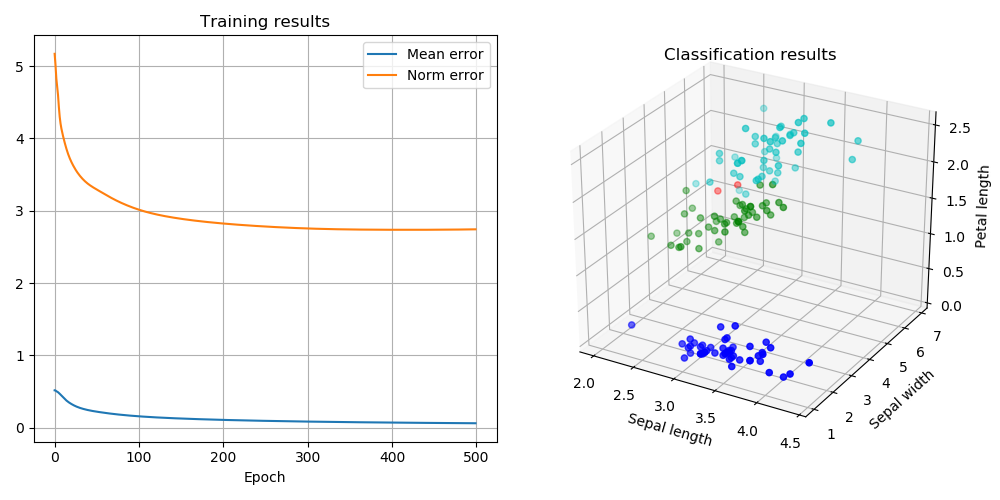
\includegraphics[scale=0.47]{LayeredNetworkIris.png}

We see that even with this more advanced network architectures, a few samples cannot be correctly classified (one or two for most training runs) because they are too close to instances of other species in the feature space. What happens if we increase the number of neurons and layers further?  The following diagram shows the results of a training run with large network with five hidden layers, having 500, 400, 300, 200 and 100 units, and a learning rate of 0.00005, where after step 3.200, the network did correctly classify all samples.

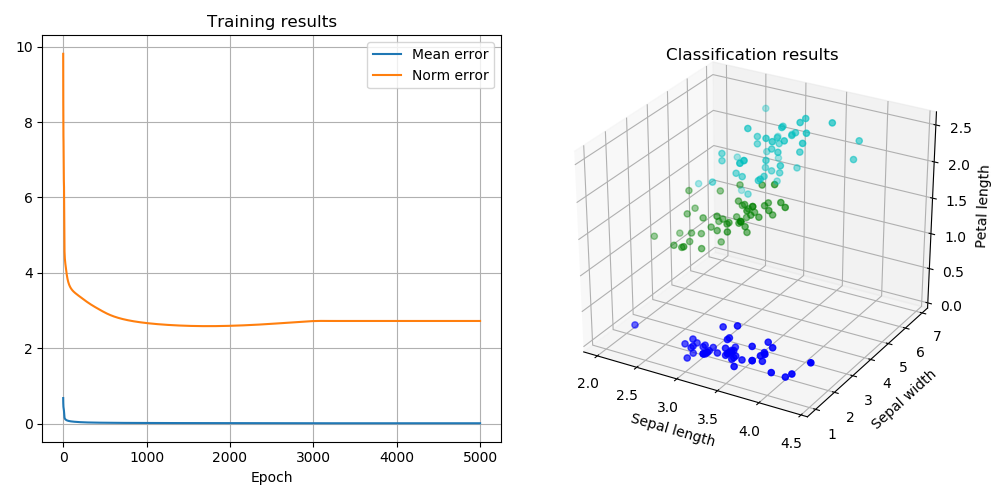
\includegraphics[scale=0.47]{LayeredNetworkIrisLarge.png}

Intuitively, the network will use the large number of individual neurons to simply remember all possible samples and the correct labels, and not create any rules. This is a typical example of {\em overtraining} that occurs if the number of free parameters that are available is much higher than the number of features in the sample set. The network will then achieve a perfect match on the training set, but will perform poorly on any new samples. Sometimes, the technique of regularization that we touch upon in then next chapter can be used to avoid overtraining.

\chapter{A few ideas from Bayesian inference}
\label{chap:ideasfrombayesianinference}

So far we have essentially employed one tool from mathematical statistics, namely the maximum likelihood estimator, to derive the weights of our neuronal networks. In this chapter, we will take a brief look at some ideas that come into play when we apply Bayesian inference to the statistical models considered so far.

As a starting point, let us go back to the logistic regression. So far, we have motivated the usage of the sigmoid function by the need for a function that maps the full real line into the unit interval to construct probabilities. However, there is an approach that leads us to the sigmoid function in a more natural way. To illustrate this, suppose we are given a scalar random variable $X$ and suspect that a binary random variable $Y$ depends on $X$. Let us assume that the data points for each class $Y = 0,1$ are both distributed according to a Gaussian distribution with a given mean and variance, i.e. that the distribution of $X$ conditioned on $Y$ is given by
$$
P(X = x | Y = 0) =  \frac{1}{\sqrt{2\pi} \sigma} e^{- \frac{(x - \mu_0)^2}{2\sigma^2}} 
$$
and similarly
$$
P(X = x | Y = 1) =  \frac{1}{\sqrt{2\pi} \sigma} e^{- \frac{(x - \mu_1)^2}{2\sigma^2}} 
$$
where we have assumed that both distributions have the same variance. Let $\pi = P(Y = 1)$ denote the a priori probability for $Y$ to be one. Then we can use Bayes theorem to calculate the probability that a given sample falls into class $Y = 1$ given $X$:
\begin{align*}
P(Y=1 | X = x) &= \frac{P(X = x | Y = 1)P(Y=1)}{P(X = x)} \\
&= \frac{\pi P(X = x | Y = 1)}{(1 - \pi)P(X = x | Y = 0) + \pi (X = x | Y = 1)} \\
&= \frac{1}{1 + \frac{1-\pi}{\pi} \frac{P(X = x | Y = 0)}{P(X = x | Y = 1)}} \\
&= \frac{1}{1 + \frac{1-\pi}{\pi} e^{- \frac{1}{2\sigma^2} (\mu_0^2 - \mu_1^2 + 2 x(\mu_1 - \mu_0))}}
\end{align*} 
This looks complicated, but it is in fact a sigmoid function. If we let 
$$
w = \frac{1}{\sigma^2} (\mu_1 - \mu_0)
$$
and
$$
b =  \frac{1}{2\sigma^2}(\mu_0^2 - \mu_1^2) - \ln \frac{1-\pi}{\pi}
$$
then we obtain
$$
P(Y = 1 | X = x) = \frac{1}{1 + e^{-(wx + b)}} = \sigma(wx + b)
$$
Thus we see that our assumption has lead us directly to a model where the conditional probability of $Y$ is described by a sigmoid function. We also obtain a nice interpretation of the parameters $w$ and $b$. The weight vector $w$ is proportional to the vector connecting the centre of the cluster of points for which $Y = 1$ with the centre of the cluster of points where $Y = 0$. The second term in the bias accounts for the fact that the a priori probabilities for $Y$ to be $1$ or $0$ are different. Note that the assumption of equal variance for both distributions makes sure that the term quadratic in $x$ cancels and we obtain a linear model. 

The distributions $P(X = x | Y)$ which we did assume to be Gaussian are often called {\em class conditional densities}, and the prior distribution of $Y$ which is given by $\pi$ in our case is called the {\em class prior}. We now have two different approaches to fit our model to training data. First, we could determine values for the parameters $w$ and $b$ using the maximum likelihood approach and we are back in the logistic regression model. This requires a fitting of two parameters in order to make predictions on the outcome for future samples. Second, we could try to fit the parameters $\pi$, $\mu_0, \mu_1$ and $\sigma$ directly. This requires the fitting of four parameters, but comes with the additional benefit that once we have these parameters, we could also create additional data which is not contained in the training set. Therefore this approach is sometimes called the {\em generative model approach}. 

Even if we use the approach of the logistic regression model to fit the parameters $w$ and $b$, we can gain additional insights by applying Bayesian methods to our problem. We could, for instance, treat $w$ as a random variable (we now ignore $b$ again as we have seen that a bias can always be modelled using an additional input dimension) and assume a prior distribution $p(w)$. Then, we can again apply Bayes theorem to calculate the a posteriori distribution of $w$ given some training data $\mathcal D$. We obtain
$$
P(w | {\mathcal D}) = \frac{P({\mathcal D} | w) P(w)}{P({\mathcal D})}
$$
The first term in the numerator is the likelihood $L(w)$ given the data. The second term is the prior distribution of $w$. The term in the denominator is a constant that does not depend on $w$. Instead of maximizing the likelihood, we could now maximize the a posteriori probability for $w$, i.e. we could try to determine the value of $w$ for which the a posteriori probability is highest. As the denominator does not depend on $w$, this amounts to minimizing
$$
- \ln L(w) - \ln P(w) = l(w) - \ln P(w)
$$
where $l(w)$ is minus the logarithmic likelihood function described earlier. This method is called the {\em MAP method} (maximum a posteriori method). Thus switching from the maximum likelihood method to MAP amounts to adding an additional term to the loss function which is minus the logarithm of the prior probability. Conversely, we see that using a maximum likelihood estimator corresponds to the assumption of a uniform distribution of $w$ (which, is course, in general not true simply because the domain of $w$ is typically unbounded and therefore a uniform distribution does not define a finite probability measure).

As an example, let us assume that the weight vector $w$ is distributed according to a Gaussian with mean zero and variance $\sigma^2$, i.e. that
$$
P(w) = \frac{1}{\sqrt{2\pi}\sigma} e^{-\frac{1}{2\sigma^2} w^2}
$$
Then our new loss function is
\begin{align}\label{eq:lossfunctionwithpenalty}
l(w) + \frac{1}{2\sigma^2} w^2 + \text{const.}
\end{align}
Thus we introduce a penalty for large values of $w$. This additional term is called a {\em regulator} in the language of neural networks. Thus a Bayesian argument does not only explain the original of the regulator but also gives us an idea on the best value, namely one half of the 
inverse of the variance, which is commonly called the {\em precision} and denoted by $\beta$. Thus, our update rule for the weights during the gradient descent process with step size $\lambda$ is now
$$
W \leftarrow W - \lambda \nabla l - \beta \lambda w
$$
Due to the minus sign, the additional term is sometimes called the {\em weight decay}. 

It is worth pointing out that this is still not a full Bayesian treatment. We still search for a single value of $w$ during the training phase of the network and then use this value for a later inference phase. In a Bayesian approach, one would treat the parameter $w$ itself as a random variable. So instead of computing
$$
P(t | w,{\mathcal D})
$$
for a fixed value of $w$ and using this to draw conclusions, one would use the relation
$$
P(t |{\mathcal D}) = \int P(t | w,{\mathcal D}) P(w | {\mathcal D}) dw
$$
and compute the {\em average} of the values $P(t | w,{\mathcal D}$ weighted by the probability $P(w | {\mathcal D})$. As a full numerical integration over $w$ is usually out of the question due to the large number of dimensions of $w$, one typically tries to replace the integral by an average over a sample. Thus, one draws a sample $w_1, \dots, w_n$ distributed according to $P(w | {\mathcal D})$, and then uses
$$
P(t |{\mathcal D}) \approx \frac{1}{n} \sum_i P(t | w_i,{\mathcal D})
$$
as an approximation, backed by the law of large numbers. Of course, in general, it is far from obvious how to generate this sample, and we will have to use a non-trivial sampling method again due to the high number of dimensions of the space in which $w$ lives. In the next section, we will see how we can apply {\em Markov chain Monte Carlo methods} to this problem.


\chapter{A simple Monte Carlo perceptron}\label{chap:MCPerceptron}

In this section, we will use a Monte-Carlo approach to sample from the space of weights of a neuronal network and use this instead of a gradient descent algorithm that determines a single maximum likelihood estimate for the best set of weights. We only discuss a very simple example and refer the reader to e.g. the work of R.~Neal (\cite{Neal1996} ) for a far more detailed and complete study.

As in the first few sections, we consider a random variable $Y$ with a conditional distribution depending on a vector $X$ (the input of the neuronal network)
and parameters $w$ (the weights) and $\alpha$ (the bias) according to
$$
P(Y = 1 | X = x) = \sigma(w^t x + \alpha)
$$
For a test sample with input values $X^{(i)} \in \R^d$ and labels $Y^{(i)} \in 
\{ 0,1 \}$, the loss function which is minus the logarithm of the likelihood  is given by
$$
l(w, \alpha) = - \ln L(w,\alpha) = -\sum_i Y^{(i)} \ln p_i - 
\sum_i (1-Y^{(i)}) \ln (1-p_i)
$$
where 
$$
p_i = \sigma(w^t x^{(i)} + \alpha)
$$
Now suppose we are given a test set ${\mathcal T}$, consisting of $N$ input vectors 
$X^{(i)}$ and corresponding labels $Y^{(i)}$. Then the likelihood function is, by definition, the probability to observe the data given values of the parameters $w$ and $\alpha$:
$$
P({\mathcal T} | w,\alpha) = L(w,\alpha) = \exp(-l(w,\alpha))
$$
Let us also assume, following the Bayesian approach, that we have a prior distribution for the parameter
$$
\Theta = (w,\alpha) \in \R^{d+1}
$$
given by some density $p(\Theta)$:
$$
P(\Theta) = p(\Theta) d\Theta
$$
where $d \Theta$ is the Lebesgue measure. Now suppose that we are given an additional test input vector $X$ and are interested in the probability that the corresponding value of $Y$ is one, i.e. in the classification result for this input. We can then write
\begin{align}\label{eq:outcomeisexpectationoverparameterspace}
P(Y=1 | X, {\mathcal T}) = \int P(Y=1 | X, \Theta) P(\Theta | {\mathcal  T}) 
\end{align}
Now the first term in the integral is simply the output of the network given some value $\Theta = (w,\alpha)$ and the input $X$. The second term is the probability of the 
parameter given the test data. According to Bayes rule, this is
\begin{align}\label{eq:conditionalparameterdensityfromlikelihood}
P(\Theta | {\mathcal T}) =
\frac{P({\mathcal T} | \Theta) P(\Theta)}{P({\mathcal T})}
= L(w,\alpha) \frac{P(\Theta)}{P({\mathcal T})}
\end{align}
Together, these equations suggest an approach how to obtain an approximation for the classification of the test data. In fact, equation \ref{eq:outcomeisexpectationoverparameterspace} presents the classification result as an expectation value over the posterior distribution of the parameter after having observed the test data. To estimate this integral, we can use a Monte Carlo method like the Metropolis-Hastings algorithm (if you have never heard of that algorithm before, I invite you to take a look at my notes \cite{christianb2018}). For that purpose, we need the conditional density for the parameter up to a constant, and equation \ref{eq:conditionalparameterdensityfromlikelihood} is
giving us exactly what we need assuming that the prior distribution $p(\Theta)$ is known. In fact, given a symmetric proposal density $q$, the acceptance probability to go from one parameter $\Theta$ to the proposed parameter $\Theta^*$ is
$$
\alpha = \min \{
1,
\frac{p(\Theta^*)L(\Theta^*)}{p(\Theta)L(\Theta)}
\}
$$
as in the Metropolis algorithm, as $q$ cancels. Let us now make a specific choice for the prior distribution - we will use a multivariate Gaussian normal distribution with variance $\sigma^2$. Thus the density is proportional to
$$
\exp(- \frac{1}{2\sigma^2} \Theta^2)
$$
Let us now define an {\em energy function} on the parameter space, given by
$$
E(\Theta) = \frac{1}{2\sigma^2} \Theta^2 + l(\Theta)
$$
(even though there is an obvious similarity with the sum of a kinetic energy and a potential energy in physics, we will see later that we should {\em not} think of the first term as a kinetic energy, but rather as an additional potential energy term).
Then
$$
\exp(-E) = p(\Theta) L(\Theta)
$$
and therefore we can write the Metropolis-Hastings acceptance probability as
$$
\alpha = \min \{1,
\exp(E(\Theta) - E(\Theta^*))
\}
$$
Thus our algorithm will proceed as follows. We start with some initial parameter value $\Theta = (w,\alpha)$ and calculate the energy $E = E(\Theta)$ for this state. Then we use this parameter as starting point for a Markov chain.  In each step, we draw a new parameter value $\Theta^* = (w^*, \alpha^*)$ from a fixed symmetric proposal density $q$ and calculate the new energy $E^* = E(\Theta^*)$. We then accept the new parameter
with probability
$$
\alpha = \min \{1,
\exp(E - E^*)
$$ 
After an initial burn-in period, we continue to sample a given number of steps. For each parameter in the sample, we then calculate the output of the neural network for our new input value $X$ and take the average of these values. This is our result for the probability that $Y = 1$. 

We remark that the energy function is nothing but the loss function including a regularization term studied in equation \eqref{eq:lossfunctionwithpenalty}. As we generate our sample according to the distribution given by the exponential of $-E$ times a normalization factor, we will draw most samples from those regions of the parameter space where this function is small, i.e. in regions close to the maximum likelihood estimate for the weights. Our algorithm basically uses a statistical path through the parameter space to explore that region. However, note that this is more than just a stochastical search of the parameter space for the point with lowest energy, as we also use sample points away from the minimum to calculate our expectation value. If we compare this with a direct scan for the weights with lowest energy, using for instance stochastic gradient descent, we see that we do not use the gradient or, put differently, we fully ignore the gradient. There are methods that use gradient information to guide the Markov chain into directions with lower energy like the Hamiltonian Monte Carlo algorithm, but we will not go deeper into this question in these notes.


As before, this algorithm can be easily programmed in a language like Python, as demonstrated in the following listing.

\begin{lstlisting}[frame=single,language=Python,caption=Monte Carlo Perceptron in Python]
prob = 0
E = energy(w, alpha)
for i in range(steps):
    w_new, alpha_new = propose(w,alpha)
    E_new = energy(w_new, alpha_new)
    if (np.random.random() <= np.exp(E - E_new)):
        w, alpha = w_new, alpha_new
        E = E_new
    #
    # If we are in the inference phase, add current 
    # value to sample
    # 
    if infer:
        prob +=  expit(np.matmul(X,w) + alpha)
return prob / steps
\end{lstlisting}

This algorithm will do a burn in (if the switch {\it infer} is false) or calculate the probability $Y = 1$ given the feature data stored in a matrix $X$ as before if
{\it infer} is true. In any case, it will run the Markov chain described above for a given number of steps. If inference is turned on, it will in addition add up the output of the Perceptron for each of the sampled positions in the variable {\it prop} so
that this number, divided by the number of steps, can be returned as an approximation for the desired classification results. 

How does this algorithm work in practice? In figure \ref{fig:MonteCarloPerceptron}, we have displayed the results of a simulation run with a Perceptron using the Monte Carlo algorithm outlined above and the Iris data set as used for the deterministic Perceptron with gradient descent. Here a prior distribution for the weights and the bias with variance $1$, i.e. a standard normal distribution, was used, with a burn-in phase of 50 steps and an inference phase with 5 steps. The diagram on the left displays the classification results. In fact, the network is able to classify all samples correctly with these parameters. The diagram on the left shows how the (two-dimensional) weights evolve over time. We see that after starting at a point close to  $(-0.4, -2.2)$, the weights move to the upper left corner of the diagram in a few steps where they then remain. The diagram in the lower part of the figure display how the loss function evolves over time. In this run, only 11 updates were accepted during the 50-step burn-in phase.


\begin{figure}[ht]
\centering
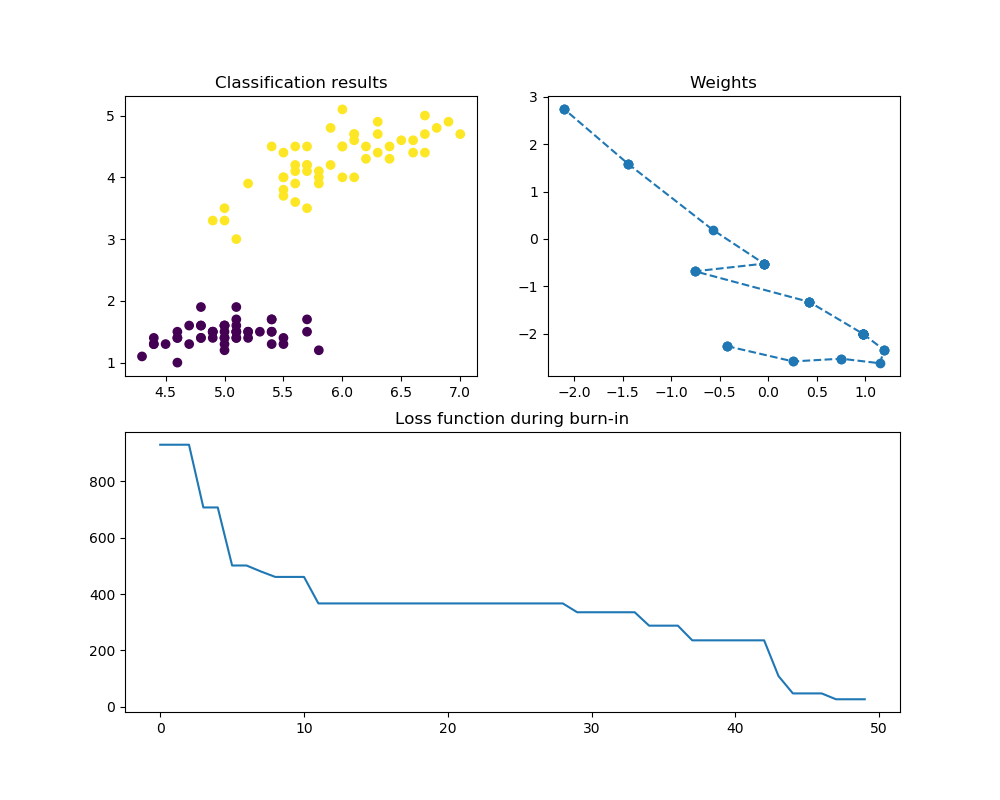
\includegraphics[scale=0.5]{MonteCarloPerceptron.png}
\caption{Monte Carlo Perceptron simulation results}
\label{fig:MonteCarloPerceptron}
\end{figure}

It is not very surprising that in this case, a Monte Carlo approach works, as the two data sets are linearly separable and any weight vector perpendicular to a line separating the classes will work. Thus it clearly suffices to be in a region close to the vector which actually minimizes the loss function, as this is what the stochastic algorithm is doing. Neal (\cite{Neal1993}, \cite{Neal1996}) has applied Monte Carlo simulations to more complex and layered networks, using not a plain Metropolis-Hastings algorithm but more sophisticated sampling methods. The approach to work with a prior distribution of the weights and then use Bayesian methods to make predictions is sometimes called {\em Bayesian neural network}. Libraries like Edward (http://edwardlib.org) which is built on top of Tensorflow or PyMC3 can assist in implementing Bayesian models that use Monte Carlo methods or what is called {\em Variational inference}, i.e. the approximation of the true posterior by simpler distributions, see also \cite{Bishop}, section 5.7 and chapter 10.

Finally, to avoid confusion, it is worth mentioning that in this example, we have applied Monte Carlo methods in the space of {\em weights}. This is very different from the large class of stochastic models known as Boltzmann machines which apply Monte Carlo methods in the space of {\em states}, but update the weights according to a classical gradient descent algorithm or variations thereof. 


%%%%%%%%%%%%%%%%%%%%%%%%%%%%%%%%%%%%%%%%%%%%%%
%% Bibliography
%%%%%%%%%%%%%%%%%%%%%%%%%%%%%%%%%%%%%%%%%%%%%%

\begin{thebibliography}{9}
	
\bibitem{Bauer}
H.~Bauer,
{\em Wahrscheinlichkeitstheorie},
de Gruyter, Berlin, New York 1991
	

\bibitem{Bishop}
C.M.~Bishop, 
{\em Pattern recognition and machine learning},
Springer, New York 2006

\bibitem{Klenke}
A.~Klenke,
{\em Probability theory}
Springer, London 2008


\bibitem{Cox}
D.R.~Cox,
{\em The regression analysis of binary sequences},
Journal of the Royal Statistical Society, Series B, Vol. 20, No. 2 (1958), pp 215--242

\bibitem{Shannon}
C.E.~Shannon,
{\em A mathematical theory of communication}, 
The Bell System Technical Journal {\em Vol. 27}, pp. 379--423, pp. 623--656, July, October 1948


\bibitem{CasellaBerger}
G.~Casella, R.L.~Berger,
{\em Statistical inference},
Duxbury Press 2002

\bibitem{Schervish}
M.J.~Schervish,
{\em Random number generation and Monte Carlo Methods},
Springer Verlag, New York, Berlin, Heidelberg 2003

\bibitem{LehmannRomano}
E.L.~Lehmann, J.P.~Romano,
{\em Testing statistical hypothesis},
Springer, New York 2005

\bibitem{Theano}
The Theano development team
{\em Theano: A Python framework for fast computation of mathematical expressions},
arXiv:1605.02688

\bibitem{Tensorflow}
M.~Abadi et.al.,
{\em TensorFlow: Large-Scale Machine Learning on Heterogeneous Distributed System},
arXiv:1603.04467

\bibitem{RHW}
D.E.~Rumelhart, G.E.~Hinton, R.J.~Williams,
{\em Learning internal representations by error propagation}, in
{\em Parallel distributed processing}, edited by D.E.~McClelland and J.L.~Rumelhart, MIT Press, 1986


\bibitem{MCMCHandbook}
S.~Brooks, A.~Gelman, C.L.~Jones,X.L.~Meng (ed.)
{\em Handbook of Markov chain Monte Carlo},
Chapman \& Hall / CRC Press, Boca Raton 2011


\bibitem{RobertCasella1999}
C.P.~Robert, G.~Casella,
{\em Monte Carlo Statistical Methods},
Springer, New York 1999


\bibitem{Neal1993}
R.M.~Neal, 
{\em Probabilist inference using Markov chain Monte Carlo methods}, 
Technical Report CRG-TR-93-1, Department of Computer Science, University of Toronto, 1993

\bibitem{Neal1996}
R.M.~Neal,
{\em Bayesian Learning for neural networks},
Springer, New York 1996

\bibitem{MacKay}
D.~MacKay,
{\em Information Theory, Inference and Learning Algorithms},
Cambridge University Press, Cambridge 2003

\bibitem{Ising1924}
E.~Ising,
{\em Beitrag zur Theorie des Ferromagnetismus},
Zeitschrift f. Physik, Vol. 31, No.1 (1924), 253--258

\bibitem{christianb2018}
C. Bohr, {\em Markov chains and Monte Carlo methods - an introduction}, available online at \url{https://github.com/christianb93/MachineLearning/blob/master/doc/MarkovChains/MarkovChainsIntroduction.pdf}

\end{thebibliography}
\end{document}


